\section{Results}
\subsection{\texttt{Gmres(m)} convergence on a larger random matrix}
Before the results from the paper are considered \texttt{gmres(m)} will be run on a random matrix of dimension $60$, the restart parameter will be varied and the effects on convergence observed. Results are shown in figure~\ref{fig:randCompM}.
In the plot a large spice is observed. In fact \texttt{gmres(34)} seems to have better convergence properties, then \texttt{gmres(35)}. 
\begin{figure}
% This file was created by matlab2tikz.
% Minimal pgfplots version: 1.3
%
%The latest updates can be retrieved from
%  http://www.mathworks.com/matlabcentral/fileexchange/22022-matlab2tikz
%where you can also make suggestions and rate matlab2tikz.
%
\documentclass[tikz]{standalone}
\usepackage{pgfplots}
\usepackage{grffile}
\pgfplotsset{compat=newest}
\usetikzlibrary{plotmarks}
\usepackage{amsmath}

\begin{document}
\definecolor{mycolor1}{rgb}{0.00000,0.44700,0.74100}%
%
\begin{tikzpicture}

\begin{axis}[%
width=2.25in,
height=2.25in,
scale only axis,
xmin=0,
xmax=50,
xlabel={inner iterations},
ymode=log,
ymin=0.461630413911085,
ymax=0.986523060510944,
yminorticks=true,
ylabel={residual}
]
\addplot [color=mycolor1,solid,forget plot]
  table[row sep=crcr]{%
1	0.986523060510944\\
2	0.985842493247835\\
3	0.951009001873142\\
4	0.933368498228608\\
5	0.930968177514434\\
6	0.919711992791358\\
7	0.913060725314143\\
8	0.908812029169852\\
9	0.901626765431656\\
10	0.901246530292743\\
11	0.897675187712453\\
12	0.892691018466368\\
13	0.888665222685472\\
14	0.886157579312595\\
15	0.885858296206797\\
16	0.885240650893534\\
17	0.869991267161745\\
18	0.840151144407451\\
19	0.814908216366823\\
20	0.815016581953242\\
21	0.811881358124345\\
22	0.808897103849879\\
23	0.809303871149252\\
24	0.809797353256798\\
25	0.793863412138822\\
26	0.795182869587702\\
27	0.764582418777165\\
28	0.763245952086273\\
29	0.764176884673488\\
30	0.754501760302079\\
31	0.755810810906755\\
32	0.754281773646681\\
33	0.739598493296359\\
34	0.631129468807206\\
35	0.736373785208064\\
36	0.732792194579432\\
37	0.732166183756903\\
38	0.728376368546021\\
39	0.611376484028501\\
40	0.584697457391735\\
41	0.591971180481715\\
42	0.589070947395509\\
43	0.57071717372384\\
44	0.512399098522211\\
45	0.527259068782117\\
46	0.525390194261684\\
47	0.509038097167017\\
48	0.511629158399782\\
49	0.507690744141563\\
50	0.461630413911085\\
};
\end{axis}
\end{tikzpicture}%
\end{document}
% This file was created by matlab2tikz.
% Minimal pgfplots version: 1.3
%
%The latest updates can be retrieved from
%  http://www.mathworks.com/matlabcentral/fileexchange/22022-matlab2tikz
%where you can also make suggestions and rate matlab2tikz.
%
\documentclass[tikz]{standalone}
\usepackage{pgfplots}
\usepackage{grffile}
\pgfplotsset{compat=newest}
\usetikzlibrary{plotmarks}
\usepackage{amsmath}

\begin{document}
\definecolor{mycolor1}{rgb}{0.00000,0.44700,0.74100}%
\definecolor{mycolor2}{rgb}{0.85000,0.32500,0.09800}%
%
\begin{tikzpicture}

\begin{axis}[%
width=1.5in,
height=1.5in,
scale only axis,
xmin=0,
xmax=1800,
xlabel={inner and outer iteratons},
ymode=log,
ymin=0.631129468807207,
ymax=1,
yminorticks=true,
ylabel={residual},
legend style={legend cell align=left,align=left,draw=white!15!black}
]
\addplot [color=mycolor1,solid]
  table[row sep=crcr]{%
1	1\\
2	0.98652369216998\\
3	0.986496833787986\\
4	0.952876445071382\\
5	0.934589397272548\\
6	0.932079691728456\\
7	0.922081971502327\\
8	0.913756212641635\\
9	0.909788525679309\\
10	0.903808987797403\\
11	0.903182755309259\\
12	0.900061274651487\\
13	0.894756037840659\\
14	0.890044536106568\\
15	0.887803991779299\\
16	0.887763093308659\\
17	0.887574438180133\\
18	0.873914668100194\\
19	0.862799840290571\\
20	0.823580620616929\\
21	0.823444599835867\\
22	0.821815992567995\\
23	0.818389196051143\\
24	0.817814932911836\\
25	0.813821638923189\\
26	0.804346981115514\\
27	0.803123242462455\\
28	0.777162696484425\\
29	0.773237780821667\\
30	0.772332232228966\\
31	0.769873431612948\\
32	0.757111922169646\\
33	0.755855095035801\\
34	0.741141136930651\\
35	0.738024056930416\\
36	0.738023937644991\\
37	0.73802327026236\\
38	0.738020030203832\\
39	0.738014049855153\\
40	0.738013920639182\\
41	0.738009244058148\\
42	0.73800227258092\\
43	0.737999893165252\\
44	0.737998465868828\\
45	0.737998072129588\\
46	0.73798385129028\\
47	0.737983846948952\\
48	0.737970788924842\\
49	0.737955041822944\\
50	0.737929210605142\\
51	0.737873548538101\\
52	0.737814630059897\\
53	0.737729225807856\\
54	0.737590135909877\\
55	0.737523871540317\\
56	0.737522702972749\\
57	0.737488131563659\\
58	0.737265643573919\\
59	0.737263777339798\\
60	0.73718624234357\\
61	0.737176961344504\\
62	0.73715144434423\\
63	0.737137622655271\\
64	0.737110021058341\\
65	0.737087705221815\\
66	0.736789572473082\\
67	0.736774538439334\\
68	0.736768199290534\\
69	0.736610437712241\\
70	0.736610422625041\\
71	0.736610398927211\\
72	0.736610198790386\\
73	0.736610191671208\\
74	0.736610174455617\\
75	0.736609327459395\\
76	0.736609288320544\\
77	0.736609288216148\\
78	0.736608822695905\\
79	0.7366083767861\\
80	0.736608297788988\\
81	0.736608258703193\\
82	0.736607906861213\\
83	0.736607712466178\\
84	0.736605288982494\\
85	0.736602623644006\\
86	0.736602294189736\\
87	0.736597924909504\\
88	0.7365910717107\\
89	0.736590946067642\\
90	0.736590838253057\\
91	0.736584072510466\\
92	0.736578951257999\\
93	0.736578000203105\\
94	0.736576906658609\\
95	0.736576756888696\\
96	0.736576589135684\\
97	0.736574371907325\\
98	0.736569041441784\\
99	0.736522683155771\\
100	0.736500423054228\\
101	0.736498363180948\\
102	0.736388331493274\\
103	0.736344131377912\\
104	0.736344129978388\\
105	0.736344122335613\\
106	0.736344049638329\\
107	0.73634396437379\\
108	0.736343961925016\\
109	0.736343775460953\\
110	0.736343466932029\\
111	0.736343453635764\\
112	0.736343396179214\\
113	0.736343362867736\\
114	0.736343059478762\\
115	0.7363430583232\\
116	0.736342769332928\\
117	0.736342349803428\\
118	0.736341419451454\\
119	0.736338113147084\\
120	0.736335649982773\\
121	0.736331588520981\\
122	0.736325095736064\\
123	0.736319612211186\\
124	0.736318524904186\\
125	0.736313955970793\\
126	0.736298711089209\\
127	0.736292604464818\\
128	0.7362921604569\\
129	0.736290554224738\\
130	0.736289986080682\\
131	0.736289819798651\\
132	0.736287241290303\\
133	0.73628520303851\\
134	0.736261600023213\\
135	0.736259743543708\\
136	0.73622460762706\\
137	0.736216620892587\\
138	0.736216620883185\\
139	0.736216620876858\\
140	0.736216609570582\\
141	0.736216587165179\\
142	0.736216586563086\\
143	0.736216575875321\\
144	0.736216456956627\\
145	0.736216453891622\\
146	0.736216453416147\\
147	0.736216414251864\\
148	0.736216406411969\\
149	0.736216376704845\\
150	0.736216335942858\\
151	0.736216229602259\\
152	0.736216073590947\\
153	0.736215598212247\\
154	0.736214832610543\\
155	0.736213779410099\\
156	0.736212775285086\\
157	0.736210732747835\\
158	0.73620953729575\\
159	0.73620851609965\\
160	0.736204359355201\\
161	0.736197178746996\\
162	0.73619717734708\\
163	0.736196772259206\\
164	0.736196651347374\\
165	0.736196651335146\\
166	0.736196230990141\\
167	0.736189109889028\\
168	0.73618803499428\\
169	0.73618784563982\\
170	0.736128904105992\\
171	0.736059344262672\\
172	0.73605933407847\\
173	0.73605932274519\\
174	0.736059283084253\\
175	0.736059272083472\\
176	0.736059269259041\\
177	0.736059119889707\\
178	0.736058943859849\\
179	0.736058939986889\\
180	0.736058871311472\\
181	0.736058788772702\\
182	0.736058784877658\\
183	0.736058784649256\\
184	0.736058743103927\\
185	0.736058587502844\\
186	0.73605793734878\\
187	0.736055679055299\\
188	0.736054094647049\\
189	0.736051275715499\\
190	0.736046602254588\\
191	0.736041043892093\\
192	0.736037182478838\\
193	0.736028441404522\\
194	0.736001090474807\\
195	0.735956000756659\\
196	0.73594371252269\\
197	0.735927118381269\\
198	0.735925299046571\\
199	0.735920788461994\\
200	0.735920119227612\\
201	0.735919757050115\\
202	0.73588633668765\\
203	0.735885720573547\\
204	0.735826434060742\\
205	0.735733147799787\\
206	0.735733073373655\\
207	0.735732982357484\\
208	0.735732975451662\\
209	0.73573297530519\\
210	0.735732934958235\\
211	0.735732849593813\\
212	0.735732642355986\\
213	0.735732636994458\\
214	0.735732558686882\\
215	0.735732284342762\\
216	0.735732240892026\\
217	0.735732228182287\\
218	0.735732216229569\\
219	0.73573220159227\\
220	0.735731974601529\\
221	0.735730458910159\\
222	0.735729461541316\\
223	0.735728214767987\\
224	0.73572550184138\\
225	0.73572042235321\\
226	0.735716516801488\\
227	0.735709409017699\\
228	0.735684880418316\\
229	0.735617319724389\\
230	0.735566342908951\\
231	0.735498500804453\\
232	0.735467152471739\\
233	0.73540554497925\\
234	0.735401427731159\\
235	0.735401009365498\\
236	0.735305963109122\\
237	0.735296954897317\\
238	0.735158886399731\\
239	0.734861077027187\\
240	0.73486013304271\\
241	0.73485901195963\\
242	0.734858916328454\\
243	0.734858684240385\\
244	0.734858163153549\\
245	0.734858099558417\\
246	0.734857640251973\\
247	0.734857628108134\\
248	0.734857142842051\\
249	0.734854721521287\\
250	0.734853584832785\\
251	0.734852707897874\\
252	0.734850899942951\\
253	0.734850354184075\\
254	0.734850292301049\\
255	0.734848829824432\\
256	0.734848413557874\\
257	0.734848191990668\\
258	0.734844791052118\\
259	0.734832499763738\\
260	0.734824118186211\\
261	0.734805254080638\\
262	0.73475828961685\\
263	0.734613961901229\\
264	0.734432012628795\\
265	0.734095252496153\\
266	0.733647554808534\\
267	0.731596856435101\\
268	0.728979696643671\\
269	0.726658482002998\\
270	0.715539337949771\\
271	0.699962029982848\\
272	0.689785038727045\\
273	0.686964540752277\\
274	0.686951498241495\\
275	0.68681514248956\\
276	0.686400674927227\\
277	0.685736223706898\\
278	0.684633184900315\\
279	0.683031600939947\\
280	0.682332611528297\\
281	0.681307353540638\\
282	0.680973083879309\\
283	0.680731981885006\\
284	0.680565965368592\\
285	0.679167900135113\\
286	0.677372079905289\\
287	0.675985468901795\\
288	0.673949943120601\\
289	0.671209515937338\\
290	0.670755090297128\\
291	0.670702378814561\\
292	0.670359578939057\\
293	0.668975367883791\\
294	0.66801818502408\\
295	0.667416982302899\\
296	0.665821722256691\\
297	0.662727850656386\\
298	0.660012023432577\\
299	0.657868153437878\\
300	0.657776975287795\\
301	0.656949579869334\\
302	0.654928599263838\\
303	0.650172481606734\\
304	0.641547127982428\\
305	0.636335751915083\\
306	0.635913894165956\\
307	0.632493985323595\\
308	0.632493122659316\\
309	0.632483709669078\\
310	0.632483682005421\\
311	0.632480842545269\\
312	0.632480837277958\\
313	0.632477991497077\\
314	0.632477783288934\\
315	0.632477613261984\\
316	0.632477611005329\\
317	0.632476866984677\\
318	0.63247491216046\\
319	0.632474165856775\\
320	0.632474155855493\\
321	0.632474003737497\\
322	0.632473999813205\\
323	0.632473100753261\\
324	0.632471747018317\\
325	0.632460434326726\\
326	0.6324601577191\\
327	0.632459319362643\\
328	0.632454386078264\\
329	0.632451217446962\\
330	0.632441302959308\\
331	0.632433319588519\\
332	0.632432648596571\\
333	0.632418063619023\\
334	0.632395840395535\\
335	0.632261636331626\\
336	0.632241179766439\\
337	0.632241115187328\\
338	0.631836002038336\\
339	0.631337551073838\\
340	0.631262123628789\\
341	0.631262011820009\\
342	0.63126201181039\\
343	0.631262006027222\\
344	0.631261962749115\\
345	0.631261961866912\\
346	0.631261961683969\\
347	0.631261955312382\\
348	0.631261952629618\\
349	0.631261948192047\\
350	0.631261920900488\\
351	0.631261871675841\\
352	0.631261858820561\\
353	0.631261833902365\\
354	0.631261712636924\\
355	0.63126171235212\\
356	0.631261684099091\\
357	0.631261672632099\\
358	0.631261656560506\\
359	0.631261634047535\\
360	0.631261620162914\\
361	0.631261425590782\\
362	0.631261422892191\\
363	0.631261277750383\\
364	0.631260977869429\\
365	0.631260634332528\\
366	0.631260458446459\\
367	0.63126011732892\\
368	0.631260002765824\\
369	0.631259963498477\\
370	0.631258382263716\\
371	0.631258311761394\\
372	0.631248890698917\\
373	0.631247928663573\\
374	0.631183097847023\\
375	0.631147409292726\\
376	0.631147405667082\\
377	0.631147365039526\\
378	0.631147364827822\\
379	0.63114731932793\\
380	0.631147270506954\\
381	0.631147220781007\\
382	0.631147175853481\\
383	0.631147127324061\\
384	0.631147116080253\\
385	0.631147112404777\\
386	0.631147099602174\\
387	0.631147084556114\\
388	0.63114700506988\\
389	0.631146970655433\\
390	0.631146970507056\\
391	0.631146906900152\\
392	0.631146897820304\\
393	0.631146717577893\\
394	0.631146717454824\\
395	0.631146705198743\\
396	0.631146673932611\\
397	0.63114661065601\\
398	0.631146512124642\\
399	0.631146478941696\\
400	0.631146471661264\\
401	0.63114647058641\\
402	0.631146451195879\\
403	0.631146450880895\\
404	0.631143694049169\\
405	0.631142668608294\\
406	0.631136228673072\\
407	0.631133298859545\\
408	0.631133163679229\\
409	0.631133147439027\\
410	0.631133147437233\\
411	0.631133147366086\\
412	0.631133147231123\\
413	0.631133147217819\\
414	0.63113314712828\\
415	0.631133146380896\\
416	0.631133145935905\\
417	0.631133145908895\\
418	0.631133142898872\\
419	0.631133140694699\\
420	0.631133140622273\\
421	0.631133138341133\\
422	0.631133135754074\\
423	0.631133135392869\\
424	0.631133134016582\\
425	0.631133133261843\\
426	0.631133128182156\\
427	0.631133127889806\\
428	0.631133124282465\\
429	0.631133119191873\\
430	0.63113311906316\\
431	0.631133098669914\\
432	0.631133098108176\\
433	0.631133077835535\\
434	0.63113307452866\\
435	0.631133073419153\\
436	0.631133073272041\\
437	0.631133070419084\\
438	0.631132971913106\\
439	0.631132891608626\\
440	0.631132840174144\\
441	0.631132641618811\\
442	0.631131361268723\\
443	0.631131101619497\\
444	0.631131101593674\\
445	0.631131101409835\\
446	0.631131101149912\\
447	0.631131099135544\\
448	0.631131097652938\\
449	0.631131097167925\\
450	0.631131094623902\\
451	0.631131092245671\\
452	0.6311310915505\\
453	0.631131091527961\\
454	0.631131090295373\\
455	0.631131088109366\\
456	0.631131085372171\\
457	0.631131084233766\\
458	0.63113108382143\\
459	0.631131081151396\\
460	0.631131080929462\\
461	0.631131075589133\\
462	0.631131075588271\\
463	0.631131075075192\\
464	0.631131073199244\\
465	0.631131071966681\\
466	0.631131068717818\\
467	0.631131068125762\\
468	0.6311310672283\\
469	0.63113106644771\\
470	0.631131063499158\\
471	0.631131057062764\\
472	0.631131015964471\\
473	0.631130976153526\\
474	0.631130767225759\\
475	0.631130750743249\\
476	0.631130741326227\\
477	0.631130680152794\\
478	0.631130680146528\\
479	0.631130680015619\\
480	0.631130679761341\\
481	0.631130679643682\\
482	0.631130679635679\\
483	0.631130679139587\\
484	0.63113067847877\\
485	0.631130678443161\\
486	0.631130678280491\\
487	0.631130677710704\\
488	0.631130677535417\\
489	0.631130677518596\\
490	0.631130677468224\\
491	0.631130677418534\\
492	0.631130676665793\\
493	0.631130676663024\\
494	0.631130675766996\\
495	0.631130675756914\\
496	0.631130674919855\\
497	0.631130674463748\\
498	0.631130674270779\\
499	0.631130671680997\\
500	0.63113067168005\\
501	0.631130669574746\\
502	0.631130667824183\\
503	0.631130666809446\\
504	0.631130665902063\\
505	0.631130665505029\\
506	0.631130646127367\\
507	0.631130617048596\\
508	0.631130615062707\\
509	0.631130605016791\\
510	0.631130523041594\\
511	0.63113050151327\\
512	0.631130501511127\\
513	0.631130501438594\\
514	0.631130501134691\\
515	0.631130500823706\\
516	0.631130500760302\\
517	0.631130500671236\\
518	0.631130499886833\\
519	0.631130499570441\\
520	0.631130499544514\\
521	0.631130499317885\\
522	0.631130498892704\\
523	0.631130498387297\\
524	0.63113049822774\\
525	0.631130498202118\\
526	0.631130497701724\\
527	0.631130497461454\\
528	0.631130497241218\\
529	0.631130496909988\\
530	0.631130496770663\\
531	0.631130496607028\\
532	0.631130496170778\\
533	0.631130495553627\\
534	0.631130495412702\\
535	0.631130495022582\\
536	0.631130493677196\\
537	0.631130492552729\\
538	0.631130491252854\\
539	0.631130488673675\\
540	0.631130488104438\\
541	0.631130471228804\\
542	0.631130455318179\\
543	0.63113045510988\\
544	0.631130435766148\\
545	0.631130369682743\\
546	0.631130369676175\\
547	0.631130369529095\\
548	0.631130369228002\\
549	0.631130369085744\\
550	0.631130369085427\\
551	0.631130368789548\\
552	0.631130368207143\\
553	0.631130368113892\\
554	0.631130368104451\\
555	0.631130367772981\\
556	0.631130367514139\\
557	0.631130367332925\\
558	0.631130367329506\\
559	0.631130367323986\\
560	0.631130366778679\\
561	0.631130366751033\\
562	0.631130366385944\\
563	0.631130366356505\\
564	0.631130366003066\\
565	0.631130365829335\\
566	0.631130365605696\\
567	0.631130364654027\\
568	0.631130364653547\\
569	0.631130363958613\\
570	0.63113036256066\\
571	0.6311303613704\\
572	0.631130360406537\\
573	0.631130359138838\\
574	0.631130351802035\\
575	0.631130334552845\\
576	0.631130332142672\\
577	0.63113033133598\\
578	0.631130303501871\\
579	0.631130254334892\\
580	0.631130254330068\\
581	0.631130254213655\\
582	0.631130253937768\\
583	0.631130253773682\\
584	0.63113025376537\\
585	0.631130253578688\\
586	0.631130253025091\\
587	0.63113025288562\\
588	0.631130252885195\\
589	0.631130252636619\\
590	0.631130252351822\\
591	0.631130252079372\\
592	0.631130252047101\\
593	0.631130252047007\\
594	0.631130251589518\\
595	0.631130251514598\\
596	0.631130251282744\\
597	0.631130251205712\\
598	0.631130250999525\\
599	0.631130250873432\\
600	0.631130250620808\\
601	0.631130250020544\\
602	0.63113025000535\\
603	0.631130249591917\\
604	0.631130248363261\\
605	0.631130247296338\\
606	0.63113024634839\\
607	0.631130244709062\\
608	0.631130241333157\\
609	0.631130227533013\\
610	0.631130222939097\\
611	0.631130222832754\\
612	0.631130203908736\\
613	0.631130150479791\\
614	0.631130150474583\\
615	0.631130150354824\\
616	0.631130150100415\\
617	0.63113014997168\\
618	0.63113014996959\\
619	0.631130149758077\\
620	0.631130149273473\\
621	0.631130149176366\\
622	0.631130149175383\\
623	0.631130148927855\\
624	0.631130148692394\\
625	0.631130148493762\\
626	0.631130148481601\\
627	0.631130148480514\\
628	0.631130148050534\\
629	0.631130148009519\\
630	0.631130147766782\\
631	0.631130147729421\\
632	0.631130147495907\\
633	0.631130147375412\\
634	0.631130147176154\\
635	0.631130146547885\\
636	0.631130146545213\\
637	0.631130146097575\\
638	0.631130144954892\\
639	0.631130143956285\\
640	0.631130143137625\\
641	0.63113014185542\\
642	0.631130137331276\\
643	0.631130124335794\\
644	0.631130121727142\\
645	0.631130121514436\\
646	0.631130102620798\\
647	0.631130057098373\\
648	0.631130057093976\\
649	0.63113005699084\\
650	0.631130056763732\\
651	0.631130056641713\\
652	0.631130056638168\\
653	0.631130056464982\\
654	0.631130056026337\\
655	0.631130055928625\\
656	0.631130055928584\\
657	0.631130055716672\\
658	0.631130055496836\\
659	0.63113005529877\\
660	0.631130055281832\\
661	0.631130055281642\\
662	0.631130054904088\\
663	0.631130054857363\\
664	0.631130054658513\\
665	0.631130054615197\\
666	0.631130054427151\\
667	0.631130054324172\\
668	0.631130054137213\\
669	0.631130053619389\\
670	0.631130053614291\\
671	0.631130053248614\\
672	0.631130052230051\\
673	0.631130051342659\\
674	0.631130050600307\\
675	0.631130049359303\\
676	0.631130045926043\\
677	0.631130034641335\\
678	0.631130031824429\\
679	0.631130031712792\\
680	0.631130015774491\\
681	0.631129973734358\\
682	0.631129973730328\\
683	0.631129973636384\\
684	0.631129973433672\\
685	0.631129973328142\\
686	0.631129973325766\\
687	0.631129973164491\\
688	0.631129972776377\\
689	0.631129972694196\\
690	0.631129972693934\\
691	0.631129972501689\\
692	0.631129972310155\\
693	0.631129972142406\\
694	0.631129972129985\\
695	0.631129972129559\\
696	0.631129971791305\\
697	0.63112997175406\\
698	0.631129971571831\\
699	0.631129971538418\\
700	0.631129971362458\\
701	0.631129971269517\\
702	0.631129971109102\\
703	0.631129970631465\\
704	0.631129970628544\\
705	0.631129970287567\\
706	0.631129969374039\\
707	0.631129968578869\\
708	0.631129967927778\\
709	0.631129966859175\\
710	0.631129963553884\\
711	0.631129953424787\\
712	0.631129951167194\\
713	0.631129951043189\\
714	0.631129936554615\\
715	0.631129899901365\\
716	0.631129899897877\\
717	0.631129899815999\\
718	0.631129899637568\\
719	0.631129899543109\\
720	0.631129899540652\\
721	0.631129899401689\\
722	0.63112989905833\\
723	0.631129898983721\\
724	0.631129898983613\\
725	0.631129898816045\\
726	0.631129898645614\\
727	0.631129898494045\\
728	0.631129898481868\\
729	0.631129898481633\\
730	0.63112989818507\\
731	0.631129898150224\\
732	0.631129897993529\\
733	0.631129897962185\\
734	0.63112989781088\\
735	0.63112989772974\\
736	0.631129897587402\\
737	0.631129897173712\\
738	0.631129897170675\\
739	0.631129896874929\\
740	0.631129896068359\\
741	0.631129895368687\\
742	0.63112989479514\\
743	0.631129893835162\\
744	0.631129891043397\\
745	0.631129882186617\\
746	0.631129880102366\\
747	0.631129880005222\\
748	0.631129867401113\\
749	0.631129835016575\\
750	0.631129835013517\\
751	0.631129834941591\\
752	0.631129834785347\\
753	0.631129834703019\\
754	0.631129834700968\\
755	0.631129834578266\\
756	0.631129834277762\\
757	0.63112983421313\\
758	0.631129834212995\\
759	0.631129834065809\\
760	0.631129833917361\\
761	0.631129833786122\\
762	0.631129833775839\\
763	0.6311298337756\\
764	0.631129833515836\\
765	0.631129833485951\\
766	0.631129833348404\\
767	0.631129833321812\\
768	0.631129833187847\\
769	0.63112983311656\\
770	0.631129832993529\\
771	0.631129832627959\\
772	0.631129832625602\\
773	0.631129832362823\\
774	0.631129831653828\\
775	0.631129831040227\\
776	0.631129830541439\\
777	0.631129829706357\\
778	0.631129827227734\\
779	0.631129819467023\\
780	0.63112981768246\\
781	0.631129817592204\\
782	0.631129806509353\\
783	0.631129778414675\\
784	0.631129778412039\\
785	0.631129778349806\\
786	0.63112977821415\\
787	0.631129778142241\\
788	0.631129778140366\\
789	0.631129778034478\\
790	0.63112977777294\\
791	0.631129777716281\\
792	0.631129777716187\\
793	0.631129777588753\\
794	0.631129777459515\\
795	0.631129777344797\\
796	0.631129777335577\\
797	0.631129777335401\\
798	0.631129777110185\\
799	0.631129777083752\\
800	0.631129776965395\\
801	0.63112977694193\\
802	0.631129776826231\\
803	0.631129776764418\\
804	0.631129776657785\\
805	0.631129776341165\\
806	0.631129776339064\\
807	0.631129776110751\\
808	0.631129775493151\\
809	0.631129774960116\\
810	0.631129774528153\\
811	0.631129773798567\\
812	0.631129771673694\\
813	0.631129764950727\\
814	0.63112976338123\\
815	0.631129763304492\\
816	0.631129753708471\\
817	0.631129729379944\\
818	0.631129729377676\\
819	0.631129729323987\\
820	0.63112972920692\\
821	0.631129729144813\\
822	0.631129729143189\\
823	0.631129729051728\\
824	0.631129728825803\\
825	0.631129728776921\\
826	0.631129728776834\\
827	0.631129728666842\\
828	0.631129728555433\\
829	0.631129728456629\\
830	0.631129728448683\\
831	0.631129728448533\\
832	0.631129728254262\\
833	0.631129728231467\\
834	0.631129728129606\\
835	0.631129728109482\\
836	0.631129728009369\\
837	0.63112972795596\\
838	0.631129727864531\\
839	0.631129727590409\\
840	0.63112972758867\\
841	0.63112972739024\\
842	0.631129726855538\\
843	0.631129726395115\\
844	0.631129726023884\\
845	0.631129725394343\\
846	0.631129723559939\\
847	0.631129717761312\\
848	0.631129716411836\\
849	0.631129716344348\\
850	0.631129708056553\\
851	0.63112968717569\\
852	0.631129687173754\\
853	0.631129687127805\\
854	0.631129687027439\\
855	0.631129686974025\\
856	0.631129686972599\\
857	0.631129686894371\\
858	0.63112968670037\\
859	0.631129686658281\\
860	0.631129686658212\\
861	0.631129686564018\\
862	0.631129686468429\\
863	0.631129686383538\\
864	0.631129686376631\\
865	0.631129686376513\\
866	0.631129686210088\\
867	0.631129686190386\\
868	0.631129686103509\\
869	0.631129686086172\\
870	0.63112968600044\\
871	0.631129685954645\\
872	0.631129685876539\\
873	0.631129685641418\\
874	0.631129685639936\\
875	0.631129685469207\\
876	0.631129685009438\\
877	0.631129684614433\\
878	0.631129684297102\\
879	0.63112968375588\\
880	0.631129682191942\\
881	0.63112967722642\\
882	0.631129676064369\\
883	0.63112967600653\\
884	0.631129668906818\\
885	0.631129651069649\\
886	0.631129651068005\\
887	0.63112965102887\\
888	0.631129650943307\\
889	0.631129650897689\\
890	0.631129650896458\\
891	0.631129650829811\\
892	0.631129650664229\\
893	0.631129650628283\\
894	0.631129650628224\\
895	0.631129650547955\\
896	0.631129650466475\\
897	0.631129650394099\\
898	0.631129650388179\\
899	0.631129650388082\\
900	0.631129650246277\\
901	0.631129650229427\\
902	0.631129650155619\\
903	0.631129650140848\\
904	0.631129650067707\\
905	0.63112965002864\\
906	0.631129649962348\\
907	0.631129649761564\\
908	0.631129649760326\\
909	0.631129649614081\\
910	0.631129649221042\\
911	0.631129648884049\\
912	0.631129648614371\\
913	0.63112964815243\\
914	0.631129646822224\\
915	0.631129642592138\\
916	0.631129641601078\\
917	0.631129641551349\\
918	0.631129635498625\\
919	0.631129620353828\\
920	0.631129620352439\\
921	0.631129620319298\\
922	0.63112962024675\\
923	0.631129620207986\\
924	0.631129620206926\\
925	0.631129620150493\\
926	0.631129620009924\\
927	0.631129619979363\\
928	0.631129619979315\\
929	0.631129619911301\\
930	0.631129619842195\\
931	0.631129619780768\\
932	0.631129619775705\\
933	0.631129619775628\\
934	0.631129619655462\\
935	0.631129619641103\\
936	0.631129619578761\\
937	0.631129619566213\\
938	0.631129619504209\\
939	0.631129619471072\\
940	0.631129619415062\\
941	0.631129619244654\\
942	0.631129619243617\\
943	0.631129619119158\\
944	0.631129618785065\\
945	0.631129618499151\\
946	0.631129618271112\\
947	0.631129617878749\\
948	0.631129616754855\\
949	0.631129613171204\\
950	0.63112961232905\\
951	0.631129612286735\\
952	0.63112960715652\\
953	0.631129594359174\\
954	0.631129594358007\\
955	0.631129594330071\\
956	0.631129594268861\\
957	0.631129594236098\\
958	0.631129594235191\\
959	0.631129594187619\\
960	0.631129594068892\\
961	0.631129594043056\\
962	0.631129594043015\\
963	0.631129593985657\\
964	0.631129593927346\\
965	0.631129593875495\\
966	0.631129593871198\\
967	0.631129593871136\\
968	0.631129593769797\\
969	0.631129593757639\\
970	0.631129593705207\\
971	0.631129593694614\\
972	0.631129593642287\\
973	0.631129593614314\\
974	0.631129593567222\\
975	0.631129593423273\\
976	0.631129593422411\\
977	0.631129593317007\\
978	0.63112959303447\\
979	0.631129592793089\\
980	0.631129592601184\\
981	0.631129592269711\\
982	0.631129591323883\\
983	0.631129588302321\\
984	0.63112958759095\\
985	0.631129587555057\\
986	0.63112958322722\\
987	0.631129572465464\\
988	0.631129572464486\\
989	0.631129572441047\\
990	0.631129572389639\\
991	0.631129572362074\\
992	0.631129572361303\\
993	0.631129572321388\\
994	0.631129572221573\\
995	0.631129572199829\\
996	0.631129572199796\\
997	0.631129572151647\\
998	0.631129572102665\\
999	0.63112957205909\\
1000	0.631129572055458\\
1001	0.631129572055408\\
1002	0.631129571970336\\
1003	0.631129571960086\\
1004	0.631129571916186\\
1005	0.631129571907279\\
1006	0.63112957186333\\
1007	0.631129571839827\\
1008	0.631129571800398\\
1009	0.631129571679384\\
1010	0.631129571678667\\
1011	0.631129571589853\\
1012	0.631129571352055\\
1013	0.631129571149215\\
1014	0.631129570988414\\
1015	0.631129570709649\\
1016	0.631129569917414\\
1017	0.631129567381382\\
1018	0.631129566783029\\
1019	0.631129566752767\\
1020	0.631129563118808\\
1021	0.631129554107109\\
1022	0.631129554106294\\
1023	0.631129554086707\\
1024	0.631129554043713\\
1025	0.631129554020623\\
1026	0.631129554019972\\
1027	0.631129553986616\\
1028	0.631129553903059\\
1029	0.631129553884841\\
1030	0.631129553884814\\
1031	0.63112955384456\\
1032	0.63112955380359\\
1033	0.631129553767129\\
1034	0.631129553764075\\
1035	0.631129553764036\\
1036	0.631129553692914\\
1037	0.631129553684313\\
1038	0.631129553647699\\
1039	0.631129553640243\\
1040	0.631129553603482\\
1041	0.631129553583817\\
1042	0.631129553550935\\
1043	0.631129553449627\\
1044	0.631129553449035\\
1045	0.631129553374527\\
1046	0.631129553175256\\
1047	0.631129553005522\\
1048	0.631129552871325\\
1049	0.63112955263791\\
1050	0.631129551976844\\
1051	0.631129549857056\\
1052	0.631129549356032\\
1053	0.631129549330621\\
1054	0.63112954629187\\
1055	0.631129538775635\\
1056	0.631129538774956\\
1057	0.631129538758651\\
1058	0.631129538722831\\
1059	0.631129538703567\\
1060	0.631129538703018\\
1061	0.63112953867525\\
1062	0.631129538605577\\
1063	0.631129538590373\\
1064	0.631129538590351\\
1065	0.631129538556828\\
1066	0.63112953852269\\
1067	0.631129538492298\\
1068	0.631129538489741\\
1069	0.631129538489709\\
1070	0.631129538430477\\
1071	0.63112953842329\\
1072	0.631129538392863\\
1073	0.631129538386646\\
1074	0.631129538356016\\
1075	0.631129538339626\\
1076	0.631129538312302\\
1077	0.631129538227828\\
1078	0.63112953822734\\
1079	0.631129538165092\\
1080	0.631129537998777\\
1081	0.631129537857298\\
1082	0.631129537745712\\
1083	0.631129537551033\\
1084	0.631129537001475\\
1085	0.63112953523635\\
1086	0.631129534818434\\
1087	0.631129534797191\\
1088	0.631129532265956\\
1089	0.63112952601954\\
1090	0.631129526018979\\
1091	0.631129526005452\\
1092	0.631129525975714\\
1093	0.6311295259597\\
1094	0.63112952595924\\
1095	0.631129525936203\\
1096	0.631129525878315\\
1097	0.631129525865674\\
1098	0.631129525865656\\
1099	0.631129525837834\\
1100	0.631129525809489\\
1101	0.631129525784249\\
1102	0.631129525782116\\
1103	0.63112952578209\\
1104	0.631129525732932\\
1105	0.631129525726949\\
1106	0.631129525701746\\
1107	0.631129525696581\\
1108	0.63112952567115\\
1109	0.631129525657538\\
1110	0.631129525634907\\
1111	0.63112952556472\\
1112	0.631129525564318\\
1113	0.631129525512508\\
1114	0.631129525374208\\
1115	0.631129525256699\\
1116	0.631129525164225\\
1117	0.631129525002443\\
1118	0.631129524547083\\
1119	0.631129523082367\\
1120	0.631129522735049\\
1121	0.631129522717357\\
1122	0.631129520616234\\
1123	0.631129515442271\\
1124	0.631129515441807\\
1125	0.631129515430621\\
1126	0.631129515406011\\
1127	0.631129515392743\\
1128	0.63112951539236\\
1129	0.631129515373308\\
1130	0.631129515325369\\
1131	0.631129515314894\\
1132	0.631129515314879\\
1133	0.631129515291862\\
1134	0.631129515268404\\
1135	0.631129515247508\\
1136	0.631129515245736\\
1137	0.631129515245716\\
1138	0.631129515205047\\
1139	0.631129515200084\\
1140	0.631129515179271\\
1141	0.631129515174994\\
1142	0.631129515153947\\
1143	0.631129515142678\\
1144	0.631129515123991\\
1145	0.631129515065867\\
1146	0.631129515065537\\
1147	0.631129515022563\\
1148	0.631129514907945\\
1149	0.631129514810662\\
1150	0.63112951473426\\
1151	0.631129514600258\\
1152	0.631129514224104\\
1153	0.631129513012521\\
1154	0.63112951272482\\
1155	0.631129512710138\\
1156	0.631129510971631\\
1157	0.631129506698866\\
1158	0.631129506698484\\
1159	0.63112950668926\\
1160	0.631129506668954\\
1161	0.631129506657994\\
1162	0.631129506657676\\
1163	0.631129506641965\\
1164	0.631129506602384\\
1165	0.63112950659373\\
1166	0.631129506593718\\
1167	0.631129506574732\\
1168	0.631129506555374\\
1169	0.631129506538127\\
1170	0.631129506536659\\
1171	0.631129506536643\\
1172	0.631129506503095\\
1173	0.631129506498991\\
1174	0.63112950648185\\
1175	0.631129506478319\\
1176	0.631129506460952\\
1177	0.631129506451651\\
1178	0.631129506436262\\
1179	0.631129506388271\\
1180	0.631129506388001\\
1181	0.631129506352467\\
1182	0.631129506257767\\
1183	0.631129506177467\\
1184	0.631129506114519\\
1185	0.631129506003862\\
1186	0.631129505693992\\
1187	0.631129504694684\\
1188	0.631129504457088\\
1189	0.631129504444942\\
1190	0.631129503010658\\
1191	0.631129499491793\\
1192	0.631129499491479\\
1193	0.631129499483893\\
1194	0.631129499467183\\
1195	0.631129499458155\\
1196	0.631129499457891\\
1197	0.631129499444969\\
1198	0.631129499412378\\
1199	0.631129499405248\\
1200	0.631129499405238\\
1201	0.631129499389618\\
1202	0.631129499373687\\
1203	0.63112949935949\\
1204	0.631129499358278\\
1205	0.631129499358265\\
1206	0.631129499330665\\
1207	0.63112949932728\\
1208	0.631129499313199\\
1209	0.631129499310291\\
1210	0.631129499295999\\
1211	0.631129499288342\\
1212	0.631129499275701\\
1213	0.631129499236184\\
1214	0.631129499235964\\
1215	0.631129499206666\\
1216	0.631129499128641\\
1217	0.631129499062538\\
1218	0.631129499010806\\
1219	0.631129498919676\\
1220	0.631129498665054\\
1221	0.631129497842995\\
1222	0.631129497647313\\
1223	0.631129497637294\\
1224	0.631129496457138\\
1225	0.631129493566365\\
1226	0.631129493566108\\
1227	0.631129493559883\\
1228	0.631129493546165\\
1229	0.631129493538748\\
1230	0.63112949353853\\
1231	0.631129493527926\\
1232	0.631129493501158\\
1233	0.631129493495298\\
1234	0.63112949349529\\
1235	0.63112949348247\\
1236	0.631129493469391\\
1237	0.631129493457733\\
1238	0.631129493456735\\
1239	0.631129493456725\\
1240	0.631129493434072\\
1241	0.631129493431288\\
1242	0.631129493419747\\
1243	0.631129493417359\\
1244	0.631129493405625\\
1245	0.631129493399338\\
1246	0.631129493388977\\
1247	0.631129493356518\\
1248	0.631129493356338\\
1249	0.631129493332246\\
1250	0.631129493268121\\
1251	0.631129493213838\\
1252	0.631129493171422\\
1253	0.63112949309656\\
1254	0.631129492887812\\
1255	0.631129492213176\\
1256	0.631129492052417\\
1257	0.631129492044175\\
1258	0.631129491075459\\
1259	0.631129488706038\\
1260	0.631129488705828\\
1261	0.631129488700731\\
1262	0.631129488689494\\
1263	0.631129488683413\\
1264	0.631129488683234\\
1265	0.631129488674552\\
1266	0.631129488652615\\
1267	0.631129488647811\\
1268	0.631129488647804\\
1269	0.631129488637305\\
1270	0.631129488626591\\
1271	0.631129488617039\\
1272	0.631129488616219\\
1273	0.631129488616211\\
1274	0.631129488597659\\
1275	0.631129488595375\\
1276	0.631129488585934\\
1277	0.631129488583977\\
1278	0.631129488574365\\
1279	0.631129488569214\\
1280	0.631129488560739\\
1281	0.631129488534139\\
1282	0.631129488533992\\
1283	0.631129488514226\\
1284	0.631129488461647\\
1285	0.63112948841717\\
1286	0.631129488382464\\
1287	0.631129488321105\\
1288	0.631129488150321\\
1289	0.631129487597868\\
1290	0.631129487466098\\
1291	0.631129487459334\\
1292	0.631129486665914\\
1293	0.6311294847278\\
1294	0.631129484727628\\
1295	0.631129484723463\\
1296	0.631129484714278\\
1297	0.631129484709303\\
1298	0.631129484709156\\
1299	0.631129484702061\\
1300	0.63112948468412\\
1301	0.631129484680189\\
1302	0.631129484680184\\
1303	0.631129484671602\\
1304	0.631129484662843\\
1305	0.631129484655033\\
1306	0.631129484654361\\
1307	0.631129484654354\\
1308	0.631129484639191\\
1309	0.631129484637321\\
1310	0.631129484629613\\
1311	0.631129484628013\\
1312	0.631129484620155\\
1313	0.631129484615943\\
1314	0.631129484609024\\
1315	0.631129484587268\\
1316	0.631129484587149\\
1317	0.631129484570967\\
1318	0.631129484527945\\
1319	0.631129484491576\\
1320	0.631129484463232\\
1321	0.631129484413044\\
1322	0.631129484273581\\
1323	0.63112948382207\\
1324	0.631129483714283\\
1325	0.631129483708744\\
1326	0.631129483060187\\
1327	0.631129481477811\\
1328	0.63112948147767\\
1329	0.631129481474273\\
1330	0.631129481466777\\
1331	0.631129481462715\\
1332	0.631129481462594\\
1333	0.631129481456807\\
1334	0.631129481442161\\
1335	0.631129481438951\\
1336	0.631129481438946\\
1337	0.631129481431945\\
1338	0.631129481424797\\
1339	0.631129481418422\\
1340	0.631129481417872\\
1341	0.631129481417867\\
1342	0.631129481405496\\
1343	0.631129481403968\\
1344	0.631129481397685\\
1345	0.631129481396379\\
1346	0.631129481389965\\
1347	0.631129481386528\\
1348	0.631129481380889\\
1349	0.631129481363128\\
1350	0.631129481363031\\
1351	0.63112948134981\\
1352	0.631129481314675\\
1353	0.631129481284989\\
1354	0.631129481261881\\
1355	0.631129481220905\\
1356	0.631129481107213\\
1357	0.631129480738856\\
1358	0.631129480650851\\
1359	0.631129480646324\\
1360	0.63112948011713\\
1361	0.631129478827368\\
1362	0.631129478827253\\
1363	0.631129478824486\\
1364	0.631129478818379\\
1365	0.631129478815068\\
1366	0.631129478814969\\
1367	0.631129478810256\\
1368	0.631129478798319\\
1369	0.631129478795702\\
1370	0.631129478795699\\
1371	0.631129478789996\\
1372	0.631129478784172\\
1373	0.631129478778977\\
1374	0.631129478778529\\
1375	0.631129478778525\\
1376	0.631129478768447\\
1377	0.6311294787672\\
1378	0.631129478762087\\
1379	0.631129478761023\\
1380	0.631129478755798\\
1381	0.631129478752997\\
1382	0.631129478748407\\
1383	0.631129478733932\\
1384	0.631129478733854\\
1385	0.63112947872307\\
1386	0.631129478694424\\
1387	0.631129478670235\\
1388	0.631129478651424\\
1389	0.631129478618026\\
1390	0.631129478525484\\
1391	0.63112947822545\\
1392	0.631129478153717\\
1393	0.631129478150023\\
1394	0.631129477718926\\
1395	0.631129476669261\\
1396	0.631129476669168\\
1397	0.631129476666918\\
1398	0.63112947666195\\
1399	0.631129476659255\\
1400	0.631129476659175\\
1401	0.631129476655341\\
1402	0.631129476645628\\
1403	0.631129476643498\\
1404	0.631129476643495\\
1405	0.631129476638856\\
1406	0.631129476634118\\
1407	0.631129476629892\\
1408	0.631129476629526\\
1409	0.631129476629523\\
1410	0.631129476621326\\
1411	0.631129476620311\\
1412	0.631129476616155\\
1413	0.631129476615289\\
1414	0.631129476611038\\
1415	0.631129476608759\\
1416	0.63112947660503\\
1417	0.63112947659325\\
1418	0.631129476593187\\
1419	0.631129476584405\\
1420	0.631129476561086\\
1421	0.631129476541405\\
1422	0.631129476526113\\
1423	0.631129476498933\\
1424	0.631129476423711\\
1425	0.631129476179681\\
1426	0.6311294761213\\
1427	0.631129476118292\\
1428	0.631129475767621\\
1429	0.63112947491453\\
1430	0.631129474914454\\
1431	0.631129474912626\\
1432	0.63112947490859\\
1433	0.6311294749064\\
1434	0.631129474906334\\
1435	0.63112947490322\\
1436	0.631129474895327\\
1437	0.631129474893595\\
1438	0.631129474893593\\
1439	0.631129474889825\\
1440	0.631129474885975\\
1441	0.631129474882541\\
1442	0.631129474882244\\
1443	0.631129474882241\\
1444	0.631129474875583\\
1445	0.631129474874757\\
1446	0.631129474871384\\
1447	0.63112947487068\\
1448	0.631129474867227\\
1449	0.631129474865375\\
1450	0.631129474862347\\
1451	0.631129474852775\\
1452	0.631129474852723\\
1453	0.631129474845582\\
1454	0.631129474826627\\
1455	0.631129474810634\\
1456	0.631129474798219\\
1457	0.63112947477613\\
1458	0.631129474715063\\
1459	0.631129474516844\\
1460	0.631129474469395\\
1461	0.631129474466948\\
1462	0.631129474182076\\
1463	0.631129473489603\\
1464	0.631129473489541\\
1465	0.631129473488058\\
1466	0.631129473484783\\
1467	0.631129473483005\\
1468	0.631129473482951\\
1469	0.631129473480426\\
1470	0.631129473474019\\
1471	0.631129473472613\\
1472	0.631129473472611\\
1473	0.631129473469554\\
1474	0.63112947346643\\
1475	0.631129473463643\\
1476	0.631129473463402\\
1477	0.631129473463399\\
1478	0.631129473457997\\
1479	0.631129473457327\\
1480	0.631129473454592\\
1481	0.63112947345402\\
1482	0.631129473451218\\
1483	0.631129473449715\\
1484	0.63112947344726\\
1485	0.631129473439491\\
1486	0.631129473439449\\
1487	0.63112947343365\\
1488	0.63112947341826\\
1489	0.631129473405281\\
1490	0.631129473395213\\
1491	0.631129473377283\\
1492	0.631129473327763\\
1493	0.631129473166945\\
1494	0.631129473128429\\
1495	0.631129473126441\\
1496	0.631129472895298\\
1497	0.631129472333828\\
1498	0.631129472333778\\
1499	0.631129472332576\\
1500	0.631129472329922\\
1501	0.63112947232848\\
1502	0.631129472328436\\
1503	0.631129472326389\\
1504	0.631129472321195\\
1505	0.631129472320055\\
1506	0.631129472320054\\
1507	0.631129472317576\\
1508	0.631129472315044\\
1509	0.631129472312784\\
1510	0.631129472312588\\
1511	0.631129472312587\\
1512	0.631129472308208\\
1513	0.631129472307664\\
1514	0.631129472305449\\
1515	0.631129472304985\\
1516	0.631129472302714\\
1517	0.631129472301495\\
1518	0.631129472299507\\
1519	0.631129472293208\\
1520	0.631129472293174\\
1521	0.63112947228847\\
1522	0.631129472275989\\
1523	0.631129472265467\\
1524	0.631129472257311\\
1525	0.631129472242773\\
1526	0.631129472202658\\
1527	0.631129472072323\\
1528	0.631129472041093\\
1529	0.63112947203948\\
1530	0.631129471852134\\
1531	0.631129471397342\\
1532	0.631129471397302\\
1533	0.631129471396329\\
1534	0.631129471394179\\
1535	0.631129471393011\\
1536	0.631129471392976\\
1537	0.631129471391319\\
1538	0.631129471387111\\
1539	0.631129471386188\\
1540	0.631129471386187\\
1541	0.63112947138418\\
1542	0.63112947138213\\
1543	0.6311294713803\\
1544	0.631129471380141\\
1545	0.63112947138014\\
1546	0.631129471376594\\
1547	0.631129471376154\\
1548	0.631129471374361\\
1549	0.631129471373986\\
1550	0.631129471372146\\
1551	0.631129471371159\\
1552	0.63112947136955\\
1553	0.631129471364448\\
1554	0.631129471364421\\
1555	0.631129471360609\\
1556	0.631129471350498\\
1557	0.631129471341977\\
1558	0.631129471335375\\
1559	0.6311294713236\\
1560	0.631129471291133\\
1561	0.631129471185604\\
1562	0.631129471160307\\
1563	0.631129471159\\
1564	0.631129471007299\\
1565	0.631129470639249\\
1566	0.631129470639217\\
1567	0.63112947063843\\
1568	0.631129470636691\\
1569	0.631129470635746\\
1570	0.631129470635717\\
1571	0.631129470634377\\
1572	0.631129470630972\\
1573	0.631129470630225\\
1574	0.631129470630224\\
1575	0.631129470628601\\
1576	0.631129470626942\\
1577	0.631129470625461\\
1578	0.631129470625333\\
1579	0.631129470625331\\
1580	0.631129470622463\\
1581	0.631129470622106\\
1582	0.631129470620657\\
1583	0.631129470620353\\
1584	0.631129470618865\\
1585	0.631129470618066\\
1586	0.631129470616765\\
1587	0.631129470612637\\
1588	0.631129470612615\\
1589	0.631129470609529\\
1590	0.631129470601345\\
1591	0.63112947059445\\
1592	0.631129470589111\\
1593	0.631129470579582\\
1594	0.631129470553327\\
1595	0.631129470467956\\
1596	0.631129470447484\\
1597	0.631129470446426\\
1598	0.631129470323696\\
1599	0.631129470026087\\
1600	0.631129470026059\\
1601	0.631129470025423\\
1602	0.631129470024017\\
1603	0.631129470023253\\
1604	0.63112947002323\\
1605	0.631129470022146\\
1606	0.631129470019393\\
1607	0.631129470018789\\
1608	0.631129470018788\\
1609	0.631129470017476\\
1610	0.631129470016135\\
1611	0.631129470014938\\
1612	0.631129470014834\\
1613	0.631129470014833\\
1614	0.631129470012514\\
1615	0.631129470012226\\
1616	0.631129470011054\\
1617	0.631129470010809\\
1618	0.631129470009606\\
1619	0.63112947000896\\
1620	0.631129470007909\\
1621	0.63112947000457\\
1622	0.631129470004553\\
1623	0.631129470002057\\
1624	0.631129469995438\\
1625	0.631129469989864\\
1626	0.631129469985549\\
1627	0.631129469977844\\
1628	0.631129469956628\\
1629	0.631129469887619\\
1630	0.631129469871065\\
1631	0.631129469870209\\
1632	0.631129469770994\\
1633	0.631129469530521\\
1634	0.631129469530498\\
1635	0.631129469529984\\
1636	0.631129469528849\\
1637	0.631129469528231\\
1638	0.631129469528212\\
1639	0.631129469527337\\
1640	0.631129469525113\\
1641	0.631129469524624\\
1642	0.631129469524624\\
1643	0.631129469523564\\
1644	0.631129469522481\\
1645	0.631129469521514\\
1646	0.631129469521429\\
1647	0.631129469521429\\
1648	0.631129469519556\\
1649	0.631129469519322\\
1650	0.631129469518377\\
1651	0.631129469518178\\
1652	0.631129469517206\\
1653	0.631129469516685\\
1654	0.631129469515836\\
1655	0.631129469513139\\
1656	0.631129469513125\\
1657	0.631129469511107\\
1658	0.631129469505759\\
1659	0.631129469501255\\
1660	0.631129469497771\\
1661	0.631129469491545\\
1662	0.631129469474412\\
1663	0.631129469418668\\
1664	0.631129469405292\\
1665	0.6311294694046\\
1666	0.631129469324452\\
1667	0.631129469130273\\
1668	0.631129469130254\\
1669	0.631129469129839\\
1670	0.631129469128922\\
1671	0.631129469128423\\
1672	0.631129469128408\\
1673	0.631129469127702\\
1674	0.631129469125906\\
1675	0.631129469125512\\
1676	0.631129469125511\\
1677	0.631129469124656\\
1678	0.631129469123781\\
1679	0.631129469123\\
1680	0.631129469122932\\
1681	0.631129469122931\\
1682	0.631129469121419\\
1683	0.631129469121231\\
1684	0.631129469120468\\
1685	0.631129469120308\\
1686	0.631129469119523\\
1687	0.631129469119102\\
1688	0.631129469118417\\
1689	0.631129469116239\\
1690	0.631129469116227\\
1691	0.631129469114597\\
1692	0.631129469110279\\
1693	0.631129469106642\\
1694	0.63112946910383\\
1695	0.631129469098803\\
1696	0.631129469084975\\
1697	0.631129469039975\\
1698	0.631129469029174\\
1699	0.631129469028615\\
1700	0.631129468963911\\
1701	0.631129468807207\\
};
\addlegendentry{GMRES(\texttt{34})};

\addplot [color=mycolor2,solid]
  table[row sep=crcr]{%
1	1\\
2	0.98652369216998\\
3	0.986496833787986\\
4	0.952876445071382\\
5	0.934589397272548\\
6	0.932079691728456\\
7	0.922081971502327\\
8	0.913756212641635\\
9	0.909788525679309\\
10	0.903808987797403\\
11	0.903182755309259\\
12	0.900061274651487\\
13	0.894756037840659\\
14	0.890044536106568\\
15	0.887803991779299\\
16	0.887763093308659\\
17	0.887574438180133\\
18	0.873914668100194\\
19	0.862799840290571\\
20	0.823580620616929\\
21	0.823444599835867\\
22	0.821815992567995\\
23	0.818389196051143\\
24	0.817814932911836\\
25	0.813821638923189\\
26	0.804346981115514\\
27	0.803123242462455\\
28	0.777162696484425\\
29	0.773237780821667\\
30	0.772332232228966\\
31	0.769873431612948\\
32	0.757111922169646\\
33	0.755855095035801\\
34	0.741141136930651\\
35	0.738024056930416\\
36	0.737985243963615\\
37	0.737985242609353\\
38	0.737985242536677\\
39	0.737981763892511\\
40	0.737977669347264\\
41	0.737977392575158\\
42	0.737972773247619\\
43	0.73796646318204\\
44	0.737964417016227\\
45	0.737962403952038\\
46	0.73796225981537\\
47	0.737951391136336\\
48	0.737951182551832\\
49	0.737942217749282\\
50	0.737928245687697\\
51	0.737909519398118\\
52	0.7378554716374\\
53	0.737811856290097\\
54	0.737752322783171\\
55	0.737638857179453\\
56	0.737592624477822\\
57	0.737584649985342\\
58	0.737559202590987\\
59	0.737382609094225\\
60	0.737371165231934\\
61	0.737302842918094\\
62	0.737292072740563\\
63	0.73726560498303\\
64	0.737246890007\\
65	0.737215165636666\\
66	0.737192456024765\\
67	0.736877234681881\\
68	0.736861496204797\\
69	0.736859152716211\\
70	0.736670057269112\\
71	0.736647845813885\\
72	0.736647834184987\\
73	0.736647590992328\\
74	0.7366472685947\\
75	0.736647267902231\\
76	0.736646943361474\\
77	0.736645710939218\\
78	0.736645585344816\\
79	0.736645480527364\\
80	0.736645092097928\\
81	0.736644452364625\\
82	0.736644340853919\\
83	0.736644337324028\\
84	0.736643510964865\\
85	0.736642749113316\\
86	0.736637289763289\\
87	0.7366329311419\\
88	0.736632127085296\\
89	0.736620469624513\\
90	0.736610360827347\\
91	0.736610189895077\\
92	0.736609780120232\\
93	0.736602168488888\\
94	0.736599759240111\\
95	0.736598098555529\\
96	0.736597659312937\\
97	0.736597642083036\\
98	0.736597615705494\\
99	0.736597093634584\\
100	0.736591857420969\\
101	0.736542957371942\\
102	0.736532335510264\\
103	0.736521269100689\\
104	0.736467097683261\\
105	0.736460466520414\\
106	0.736453186169348\\
107	0.736453183629342\\
108	0.736453178154011\\
109	0.736453153685574\\
110	0.736453135183676\\
111	0.736453114666441\\
112	0.736453074642597\\
113	0.736452923350214\\
114	0.73645284905756\\
115	0.736452829448768\\
116	0.736452774451633\\
117	0.736452600889335\\
118	0.736452585236482\\
119	0.736452547271121\\
120	0.736452513199822\\
121	0.736452496568385\\
122	0.736451718126211\\
123	0.736451311400708\\
124	0.736451230801584\\
125	0.736450463294924\\
126	0.736449775370859\\
127	0.736449591014615\\
128	0.736449529496973\\
129	0.736447339753896\\
130	0.736447339104519\\
131	0.736446220640456\\
132	0.736445880200366\\
133	0.736445843585903\\
134	0.736445701331004\\
135	0.736444377145693\\
136	0.736443115907366\\
137	0.736426323380831\\
138	0.736425565457932\\
139	0.736419222440323\\
140	0.736412703938857\\
141	0.736411152309582\\
142	0.736411151685745\\
143	0.736411141986859\\
144	0.736411137322746\\
145	0.736411134059857\\
146	0.736411121431677\\
147	0.736411082884375\\
148	0.736411040143723\\
149	0.736411034718514\\
150	0.7364110149383\\
151	0.736410965990063\\
152	0.736410965957613\\
153	0.736410964975235\\
154	0.736410954645589\\
155	0.736410947104084\\
156	0.736410794700784\\
157	0.73641074237817\\
158	0.736410738350333\\
159	0.736410542174947\\
160	0.736410366045899\\
161	0.736410321426138\\
162	0.736410320297047\\
163	0.736410052875177\\
164	0.736410049589619\\
165	0.736409758038668\\
166	0.736409572889025\\
167	0.736409565595076\\
168	0.736409565212838\\
169	0.736409561495793\\
170	0.73640951338903\\
171	0.736405639687433\\
172	0.736405547905439\\
173	0.736404183875805\\
174	0.736399373083558\\
175	0.736399371313308\\
176	0.736397951287652\\
177	0.736397950685613\\
178	0.736397948174401\\
179	0.736397947787776\\
180	0.736397946552188\\
181	0.736397939729635\\
182	0.736397939728086\\
183	0.7363979204746\\
184	0.736397909776831\\
185	0.736397909754761\\
186	0.736397895493855\\
187	0.736397885883315\\
188	0.736397884337023\\
189	0.736397884321254\\
190	0.736397884076352\\
191	0.736397872298038\\
192	0.736397854812275\\
193	0.736397838749925\\
194	0.736397820593115\\
195	0.736397816682908\\
196	0.736397773866773\\
197	0.736397748516303\\
198	0.736397737652417\\
199	0.736397629877397\\
200	0.736397620835468\\
201	0.736397503685798\\
202	0.736397491163033\\
203	0.736397490684503\\
204	0.736397473773996\\
205	0.736397354413515\\
206	0.736396836570804\\
207	0.736395272715964\\
208	0.736395270961356\\
209	0.73639370595106\\
210	0.736393165756\\
211	0.736392579971478\\
212	0.736392579709509\\
213	0.736392577593788\\
214	0.736392577362067\\
215	0.736392576775132\\
216	0.736392573286491\\
217	0.736392569814925\\
218	0.736392560753019\\
219	0.736392558404916\\
220	0.736392556824056\\
221	0.736392547802845\\
222	0.736392547539454\\
223	0.736392547532196\\
224	0.736392546488073\\
225	0.736392545058381\\
226	0.736392522287061\\
227	0.73639252038976\\
228	0.736392518696269\\
229	0.736392486229\\
230	0.736392472421322\\
231	0.736392461742133\\
232	0.736392459160688\\
233	0.736392425118964\\
234	0.736392422433521\\
235	0.736392390807339\\
236	0.736392353032016\\
237	0.736392352858407\\
238	0.736392352580553\\
239	0.736392346320535\\
240	0.736392344424616\\
241	0.736391764144916\\
242	0.736391558460482\\
243	0.736391389225014\\
244	0.736390582074865\\
245	0.736390517157124\\
246	0.736389992205471\\
247	0.7363899919583\\
248	0.736389990707743\\
249	0.736389990696722\\
250	0.736389990536985\\
251	0.736389987802358\\
252	0.736389987222189\\
253	0.736389982957457\\
254	0.736389980298434\\
255	0.736389980208232\\
256	0.736389975775854\\
257	0.736389975024083\\
258	0.736389974554807\\
259	0.736389974108249\\
260	0.736389972795427\\
261	0.736389961926433\\
262	0.736389961924994\\
263	0.736389961440781\\
264	0.736389939925345\\
265	0.736389937395384\\
266	0.736389933643591\\
267	0.736389926924028\\
268	0.736389915542787\\
269	0.736389907442722\\
270	0.736389903848901\\
271	0.736389884612578\\
272	0.736389883886806\\
273	0.736389882268001\\
274	0.736389876135021\\
275	0.736389860784912\\
276	0.736389684874984\\
277	0.73638940122118\\
278	0.736389383419803\\
279	0.736389088503534\\
280	0.736388915147962\\
281	0.736388547946684\\
282	0.736388547765723\\
283	0.736388546644787\\
284	0.736388546484818\\
285	0.736388546431123\\
286	0.736388544394333\\
287	0.736388543112145\\
288	0.736388540916449\\
289	0.736388539571402\\
290	0.73638853931039\\
291	0.736388536360466\\
292	0.73638853633332\\
293	0.736388536049955\\
294	0.736388535066966\\
295	0.736388533128499\\
296	0.736388520740619\\
297	0.736388518788827\\
298	0.736388518696313\\
299	0.736388493291478\\
300	0.736388484700914\\
301	0.736388484301022\\
302	0.736388480842882\\
303	0.736388467745149\\
304	0.73638846747443\\
305	0.736388463997601\\
306	0.736388457446597\\
307	0.736388457440485\\
308	0.736388455666949\\
309	0.736388451019664\\
310	0.736388449484127\\
311	0.736388318486747\\
312	0.736388221788988\\
313	0.736388169948869\\
314	0.736388065684864\\
315	0.736387943040264\\
316	0.736387585463453\\
317	0.736387585278669\\
318	0.736387584258323\\
319	0.736387584071498\\
320	0.736387584069015\\
321	0.736387582127884\\
322	0.736387581142391\\
323	0.736387580053256\\
324	0.736387578766726\\
325	0.736387578687704\\
326	0.736387576689858\\
327	0.736387576686298\\
328	0.736387576093494\\
329	0.736387574879527\\
330	0.736387572289631\\
331	0.736387560582125\\
332	0.736387558119195\\
333	0.736387557191697\\
334	0.736387528808275\\
335	0.736387520108159\\
336	0.736387520017045\\
337	0.736387515427084\\
338	0.736387505693833\\
339	0.736387505661637\\
340	0.736387505228072\\
341	0.736387503060253\\
342	0.73638750291456\\
343	0.736387499913991\\
344	0.736387495394695\\
345	0.736387494185464\\
346	0.736387434942689\\
347	0.736387357457975\\
348	0.736387327406571\\
349	0.736387310273676\\
350	0.736387131643784\\
351	0.736386782597806\\
352	0.73638678240857\\
353	0.736386781305484\\
354	0.736386780943934\\
355	0.736386780938804\\
356	0.736386778989475\\
357	0.736386777618402\\
358	0.736386777058945\\
359	0.736386776007648\\
360	0.736386775919458\\
361	0.736386774305338\\
362	0.736386774247023\\
363	0.736386773499541\\
364	0.736386771660781\\
365	0.736386768062482\\
366	0.736386754125258\\
367	0.736386748888774\\
368	0.736386746196699\\
369	0.736386710636427\\
370	0.736386697323745\\
371	0.736386696104362\\
372	0.736386691790448\\
373	0.736386681595847\\
374	0.736386681051532\\
375	0.736386680939781\\
376	0.736386680710402\\
377	0.736386680629457\\
378	0.736386676715089\\
379	0.736386672132429\\
380	0.736386672132427\\
381	0.736386632895148\\
382	0.736386593068289\\
383	0.736386551643869\\
384	0.736386551397731\\
385	0.736386344719536\\
386	0.736385961308636\\
387	0.736385961089886\\
388	0.736385959848698\\
389	0.736385959330776\\
390	0.736385959294764\\
391	0.73638595713899\\
392	0.736385955549449\\
393	0.736385955274023\\
394	0.736385954207361\\
395	0.736385954154281\\
396	0.736385952731752\\
397	0.736385952564291\\
398	0.736385951468634\\
399	0.736385948967304\\
400	0.73638594413508\\
401	0.736385927849918\\
402	0.736385920346974\\
403	0.736385915414792\\
404	0.736385871373725\\
405	0.736385854750694\\
406	0.73638585169842\\
407	0.736385846772808\\
408	0.736385836903843\\
409	0.736385835573726\\
410	0.736385835556882\\
411	0.736385835481439\\
412	0.736385835298657\\
413	0.736385829938516\\
414	0.73638582494336\\
415	0.736385824701034\\
416	0.736385802301651\\
417	0.736385773555485\\
418	0.736385731376419\\
419	0.736385711778754\\
420	0.736385444986813\\
421	0.73638501873613\\
422	0.736385018479559\\
423	0.736385017023033\\
424	0.736385016281459\\
425	0.73638501620006\\
426	0.736385013764894\\
427	0.736385011757321\\
428	0.736385011621905\\
429	0.736385010554335\\
430	0.736385010507205\\
431	0.736385009118489\\
432	0.736385008752439\\
433	0.736385007322257\\
434	0.736385003968617\\
435	0.736384997690203\\
436	0.736384978097197\\
437	0.736384967501038\\
438	0.736384959959868\\
439	0.736384905953788\\
440	0.736384884968856\\
441	0.736384879912857\\
442	0.736384874851246\\
443	0.736384864752986\\
444	0.736384862290894\\
445	0.73638486219708\\
446	0.73638486132464\\
447	0.736384861077241\\
448	0.736384854321722\\
449	0.736384848779982\\
450	0.736384847592485\\
451	0.736384832114084\\
452	0.736384813122403\\
453	0.73638476200776\\
454	0.736384705136187\\
455	0.736384385843713\\
456	0.736383907318425\\
457	0.7363839070138\\
458	0.736383905323429\\
459	0.736383904368713\\
460	0.736383904232228\\
461	0.736383901473405\\
462	0.736383899107994\\
463	0.73638389904321\\
464	0.73638389792849\\
465	0.736383897893854\\
466	0.736383896470504\\
467	0.736383895900735\\
468	0.73638389408784\\
469	0.736383889885105\\
470	0.736383882151072\\
471	0.736383859418743\\
472	0.736383846211407\\
473	0.736383836175564\\
474	0.736383772863576\\
475	0.736383748688302\\
476	0.736383741986153\\
477	0.736383736855141\\
478	0.73638372706424\\
479	0.736383723966607\\
480	0.736383723789761\\
481	0.736383721663151\\
482	0.736383721279359\\
483	0.73638371310318\\
484	0.736383707015761\\
485	0.736383704902382\\
486	0.736383694084289\\
487	0.736383679189396\\
488	0.736383622168682\\
489	0.736383523519824\\
490	0.736383152621576\\
491	0.736382631270793\\
492	0.736382630919396\\
493	0.736382629011909\\
494	0.736382627861888\\
495	0.736382627673739\\
496	0.736382624639999\\
497	0.736382621949732\\
498	0.73638262191751\\
499	0.736382620785885\\
500	0.736382620758914\\
501	0.736382619267663\\
502	0.736382618485623\\
503	0.736382616357751\\
504	0.736382611400951\\
505	0.73638260244237\\
506	0.736382577136967\\
507	0.736382561844891\\
508	0.736382549844331\\
509	0.73638247962498\\
510	0.736382453478855\\
511	0.736382445884675\\
512	0.736382441107554\\
513	0.736382431988057\\
514	0.736382428637971\\
515	0.736382428481293\\
516	0.736382425014707\\
517	0.73638242450378\\
518	0.736382415290697\\
519	0.736382408831614\\
520	0.736382405861865\\
521	0.736382397266529\\
522	0.736382385158416\\
523	0.73638232209542\\
524	0.736382189654411\\
525	0.736381787862206\\
526	0.736381243462027\\
527	0.736381243073653\\
528	0.736381241026418\\
529	0.736381239755259\\
530	0.736381239527409\\
531	0.736381236339818\\
532	0.73638123348803\\
533	0.736381233470159\\
534	0.73638123235516\\
535	0.736381232336519\\
536	0.736381230793808\\
537	0.736381229854219\\
538	0.736381227520497\\
539	0.736381222092857\\
540	0.736381212419818\\
541	0.736381185932535\\
542	0.736381169784856\\
543	0.736381156789993\\
544	0.736381083986868\\
545	0.736381057974622\\
546	0.73638105041437\\
547	0.736381046260574\\
548	0.736381038323772\\
549	0.736381035258777\\
550	0.736381035164923\\
551	0.736381030675878\\
552	0.736381030040895\\
553	0.736381020342211\\
554	0.736381013834496\\
555	0.736381010516197\\
556	0.736381003256968\\
557	0.736380992427387\\
558	0.736380927244859\\
559	0.736380776964951\\
560	0.736380369238706\\
561	0.736379832037507\\
562	0.736379831632719\\
563	0.736379829562574\\
564	0.736379828266266\\
565	0.736379828020167\\
566	0.736379824859549\\
567	0.736379822033875\\
568	0.736379822021309\\
569	0.736379820977162\\
570	0.736379820965007\\
571	0.736379819420845\\
572	0.736379818401133\\
573	0.736379816034903\\
574	0.736379810524395\\
575	0.73637980082685\\
576	0.736379774878372\\
577	0.736379759182351\\
578	0.736379746353162\\
579	0.736379676077819\\
580	0.736379652134049\\
581	0.736379645425098\\
582	0.736379642096016\\
583	0.736379635610402\\
584	0.736379633136437\\
585	0.736379633109252\\
586	0.736379628157088\\
587	0.736379627453612\\
588	0.736379617985296\\
589	0.736379611810987\\
590	0.736379608612854\\
591	0.736379602006002\\
592	0.736379591950973\\
593	0.736379528334623\\
594	0.736379379381625\\
595	0.736378994973673\\
596	0.736378496037586\\
597	0.736378495641919\\
598	0.736378493682006\\
599	0.736378492465848\\
600	0.736378492225294\\
601	0.736378489281725\\
602	0.73637848668251\\
603	0.736378486670852\\
604	0.736378485742409\\
605	0.736378485735292\\
606	0.736378484261269\\
607	0.736378483260171\\
608	0.736378481037293\\
609	0.736378475860848\\
610	0.73637846684275\\
611	0.736378443139686\\
612	0.736378429107257\\
613	0.736378417504181\\
614	0.736378354396657\\
615	0.736378334012275\\
616	0.736378328646253\\
617	0.73637832615558\\
618	0.736378321174678\\
619	0.736378319413539\\
620	0.736378319413305\\
621	0.73637831463567\\
622	0.736378313929623\\
623	0.736378305333274\\
624	0.736378299831971\\
625	0.736378297171375\\
626	0.736378290963498\\
627	0.736378281328781\\
628	0.736378223407552\\
629	0.73637809201582\\
630	0.736377754061608\\
631	0.736377318215087\\
632	0.736377317853065\\
633	0.736377316115572\\
634	0.736377315061309\\
635	0.736377314846926\\
636	0.736377312272574\\
637	0.736377310044321\\
638	0.736377310031001\\
639	0.736377309248091\\
640	0.736377309244205\\
641	0.736377307909665\\
642	0.736377307011541\\
643	0.736377305074647\\
644	0.736377300561791\\
645	0.736377292761351\\
646	0.736377272519791\\
647	0.736377260902424\\
648	0.736377251226862\\
649	0.736377198313235\\
650	0.736377182141185\\
651	0.736377178235722\\
652	0.73637717648126\\
653	0.736377172842616\\
654	0.736377171724057\\
655	0.736377171709419\\
656	0.736377167607945\\
657	0.736377166967995\\
658	0.736377159686903\\
659	0.736377155068863\\
660	0.736377153129348\\
661	0.736377147208426\\
662	0.736377137958438\\
663	0.736377088464313\\
664	0.73637698418048\\
665	0.736376706209837\\
666	0.736376346619612\\
667	0.736376346308469\\
668	0.736376344861101\\
669	0.736376344012678\\
670	0.736376343836838\\
671	0.736376341713963\\
672	0.736376339926566\\
673	0.736376339910062\\
674	0.736376339280355\\
675	0.73637633927834\\
676	0.736376338132478\\
677	0.736376337391589\\
678	0.73637633581672\\
679	0.736376332146617\\
680	0.736376325835479\\
681	0.736376309594377\\
682	0.736376300631614\\
683	0.736376293135859\\
684	0.736376251445994\\
685	0.73637623939822\\
686	0.736376236787366\\
687	0.736376235603459\\
688	0.736376233044036\\
689	0.736376232412108\\
690	0.736376232360869\\
691	0.736376229193229\\
692	0.736376228663522\\
693	0.736376222867241\\
694	0.736376219191135\\
695	0.736376217959556\\
696	0.736376212361159\\
697	0.736376203556364\\
698	0.736376163735264\\
699	0.736376088626643\\
700	0.736375873090313\\
701	0.736375591073953\\
702	0.736375590821181\\
703	0.736375589680583\\
704	0.736375589041835\\
705	0.736375588907907\\
706	0.736375587246197\\
707	0.73637558589399\\
708	0.736375585873684\\
709	0.736375585387344\\
710	0.736375585386279\\
711	0.736375584449075\\
712	0.736375583881741\\
713	0.736375582678203\\
714	0.73637557987231\\
715	0.73637557505872\\
716	0.736375562718824\\
717	0.736375556217067\\
718	0.736375550774586\\
719	0.736375519649095\\
720	0.736375511136301\\
721	0.736375509520253\\
722	0.736375508743075\\
723	0.736375506984621\\
724	0.736375506669591\\
725	0.736375506581229\\
726	0.736375504359912\\
727	0.736375503956297\\
728	0.736375499582867\\
729	0.736375496783198\\
730	0.73637549610955\\
731	0.736375490913824\\
732	0.736375482694765\\
733	0.73637545226114\\
734	0.736375402876671\\
735	0.736375244033545\\
736	0.736375032046893\\
737	0.736375031851139\\
738	0.736375030993746\\
739	0.736375030540109\\
740	0.736375030444444\\
741	0.736375029199418\\
742	0.736375028226515\\
743	0.736375028202744\\
744	0.736375027839013\\
745	0.7363750278384\\
746	0.73637502710322\\
747	0.736375026696284\\
748	0.736375025824002\\
749	0.736375023789515\\
750	0.73637502029729\\
751	0.736375011340779\\
752	0.736375006866414\\
753	0.736375003128778\\
754	0.736374980904663\\
755	0.736374975144323\\
756	0.736374974212601\\
757	0.736374973708401\\
758	0.736374972514106\\
759	0.736374972379748\\
760	0.736374972266919\\
761	0.736374970843305\\
762	0.736374970556948\\
763	0.736374967399035\\
764	0.736374965339883\\
765	0.736374965034622\\
766	0.736374960333299\\
767	0.736374952833859\\
768	0.736374930555871\\
769	0.73637490081307\\
770	0.736374788518752\\
771	0.736374634472738\\
772	0.736374634326907\\
773	0.736374633706545\\
774	0.736374633399886\\
775	0.736374633335186\\
776	0.736374632434408\\
777	0.736374631762502\\
778	0.736374631736346\\
779	0.736374631470829\\
780	0.736374631470417\\
781	0.736374630912882\\
782	0.736374630636797\\
783	0.736374630031721\\
784	0.736374628619557\\
785	0.736374626187035\\
786	0.736374619919705\\
787	0.736374616971803\\
788	0.736374614522125\\
789	0.736374599205118\\
790	0.736374595436805\\
791	0.73637459493522\\
792	0.73637459460812\\
793	0.736374593798464\\
794	0.73637459375309\\
795	0.736374593631271\\
796	0.736374592794458\\
797	0.736374592603426\\
798	0.736374590400792\\
799	0.736374588924805\\
800	0.73637458882108\\
801	0.736374584676762\\
802	0.73637457799908\\
803	0.736374562231684\\
804	0.736374545840538\\
805	0.736374469013201\\
806	0.736374359883867\\
807	0.736374359778419\\
808	0.73637435934255\\
809	0.736374359143539\\
810	0.736374359101727\\
811	0.736374358467012\\
812	0.736374358017709\\
813	0.736374357990626\\
814	0.736374357800055\\
815	0.736374357799731\\
816	0.736374357387713\\
817	0.736374357208957\\
818	0.736374356803587\\
819	0.736374355856748\\
820	0.73637435421528\\
821	0.736374349950309\\
822	0.736374348075388\\
823	0.736374346530393\\
824	0.736374336252036\\
825	0.736374333848851\\
826	0.736374333597348\\
827	0.736374333383313\\
828	0.736374332831953\\
829	0.736374332822455\\
830	0.736374332704253\\
831	0.736374332253746\\
832	0.736374332132755\\
833	0.736374330635525\\
834	0.736374329596184\\
835	0.736374329577634\\
836	0.736374326014848\\
837	0.736374320206517\\
838	0.736374309326282\\
839	0.736374301128195\\
840	0.736374249835622\\
841	0.736374173898485\\
842	0.736374173823867\\
843	0.736374173524065\\
844	0.736374173399087\\
845	0.736374173373059\\
846	0.736374172934112\\
847	0.736374172640827\\
848	0.736374172614267\\
849	0.736374172478965\\
850	0.736374172478678\\
851	0.73637417217981\\
852	0.736374172068444\\
853	0.736374171803975\\
854	0.736374171185605\\
855	0.736374170103685\\
856	0.736374167258777\\
857	0.736374166098909\\
858	0.736374165154345\\
859	0.736374158386766\\
860	0.736374156881721\\
861	0.736374156765469\\
862	0.736374156623558\\
863	0.73637415624503\\
864	0.736374156244825\\
865	0.736374156138033\\
866	0.73637415591795\\
867	0.736374155844626\\
868	0.736374154845063\\
869	0.736374154121263\\
870	0.736374154121236\\
871	0.736374151126261\\
872	0.736374146182798\\
873	0.736374138806014\\
874	0.736374135163665\\
875	0.736374101501517\\
876	0.736374049262002\\
877	0.736374049209962\\
878	0.736374049006657\\
879	0.736374048930177\\
880	0.736374048914458\\
881	0.736374048614543\\
882	0.736374048426331\\
883	0.736374048401469\\
884	0.73637404830598\\
885	0.73637404830571\\
886	0.736374048091593\\
887	0.736374048024363\\
888	0.736374047855091\\
889	0.73637404745881\\
890	0.736374046757231\\
891	0.736374044884379\\
892	0.736374044181973\\
893	0.736374043618666\\
894	0.736374039217242\\
895	0.73637403828592\\
896	0.736374038237553\\
897	0.736374038142035\\
898	0.736374037879666\\
899	0.736374037877844\\
900	0.736374037786033\\
901	0.736374037690765\\
902	0.736374037647967\\
903	0.736374036988181\\
904	0.736374036487044\\
905	0.736374036475674\\
906	0.736374034006713\\
907	0.736374029880236\\
908	0.736374024934366\\
909	0.736374023566616\\
910	0.73637400171329\\
911	0.736373965996499\\
912	0.736373965960518\\
913	0.736373965823787\\
914	0.736373965777905\\
915	0.736373965768641\\
916	0.736373965565071\\
917	0.736373965445596\\
918	0.736373965423213\\
919	0.736373965355978\\
920	0.736373965355721\\
921	0.736373965203451\\
922	0.73637396516389\\
923	0.736373965056925\\
924	0.736373964806138\\
925	0.736373964355789\\
926	0.736373963131978\\
927	0.736373962713262\\
928	0.736373962383849\\
929	0.736373959540547\\
930	0.736373958968176\\
931	0.736373958950992\\
932	0.736373958885738\\
933	0.736373958702119\\
934	0.736373958695796\\
935	0.736373958619585\\
936	0.736373958585014\\
937	0.736373958560839\\
938	0.736373958127881\\
939	0.736373957781528\\
940	0.736373957751052\\
941	0.736373955749192\\
942	0.736373952362961\\
943	0.736373949066062\\
944	0.73637394868428\\
945	0.736373934576558\\
946	0.736373910205131\\
947	0.736373910180356\\
948	0.736373910088721\\
949	0.736373910061598\\
950	0.736373910056245\\
951	0.736373909918384\\
952	0.736373909842977\\
953	0.736373909823468\\
954	0.73637390977611\\
955	0.736373909775868\\
956	0.736373909667963\\
957	0.736373909645162\\
958	0.736373909578068\\
959	0.736373909420495\\
960	0.736373909132861\\
961	0.73637390833536\\
962	0.736373908088526\\
963	0.736373907898816\\
964	0.736373906066093\\
965	0.736373905715238\\
966	0.736373905710673\\
967	0.736373905665484\\
968	0.736373905535819\\
969	0.736373905525562\\
970	0.736373905463881\\
971	0.7363739054548\\
972	0.736373905441541\\
973	0.736373905157843\\
974	0.736373904918197\\
975	0.736373904871569\\
976	0.736373903270939\\
977	0.736373900532823\\
978	0.736373898338518\\
979	0.736373898289851\\
980	0.736373889194448\\
981	0.736373872545579\\
982	0.736373872528527\\
983	0.736373872467102\\
984	0.736373872451235\\
985	0.736373872448189\\
986	0.736373872354733\\
987	0.73637387230721\\
988	0.736373872290654\\
989	0.736373872257224\\
990	0.736373872257002\\
991	0.736373872180587\\
992	0.736373872167666\\
993	0.736373872125704\\
994	0.736373872026968\\
995	0.736373871843415\\
996	0.73637387132322\\
997	0.736373871178763\\
998	0.736373871070789\\
999	0.736373869887779\\
1000	0.736373869672515\\
1001	0.736373869671967\\
1002	0.736373869640299\\
1003	0.736373869548001\\
1004	0.736373869535422\\
1005	0.736373869486417\\
1006	0.736373869485477\\
1007	0.736373869478404\\
1008	0.736373869292144\\
1009	0.736373869125805\\
1010	0.736373869069582\\
1011	0.736373867804576\\
1012	0.73637386561832\\
1013	0.736373864155309\\
1014	0.736373864152333\\
1015	0.736373858276233\\
1016	0.736373846864222\\
1017	0.736373846852462\\
1018	0.736373846811164\\
1019	0.736373846801945\\
1020	0.736373846800234\\
1021	0.736373846736662\\
1022	0.736373846706655\\
1023	0.736373846692909\\
1024	0.736373846669231\\
1025	0.736373846669033\\
1026	0.736373846614847\\
1027	0.736373846607626\\
1028	0.736373846581363\\
1029	0.736373846519438\\
1030	0.736373846402012\\
1031	0.7363738460614\\
1032	0.736373845977195\\
1033	0.736373845916287\\
1034	0.736373845149423\\
1035	0.736373845016851\\
1036	0.736373845016812\\
1037	0.736373844994394\\
1038	0.736373844928238\\
1039	0.736373844914917\\
1040	0.736373844876514\\
1041	0.736373844876328\\
1042	0.736373844872658\\
1043	0.736373844749811\\
1044	0.73637384463384\\
1045	0.736373844574492\\
1046	0.736373843584375\\
1047	0.736373841857401\\
1048	0.736373840877888\\
1049	0.736373840822092\\
1050	0.736373837007903\\
1051	0.736373829146973\\
1052	0.736373829138832\\
1053	0.736373829110926\\
1054	0.736373829105591\\
1055	0.736373829104639\\
1056	0.736373829061174\\
1057	0.736373829042138\\
1058	0.736373829030931\\
1059	0.736373829014093\\
1060	0.73637382901392\\
1061	0.736373828975394\\
1062	0.736373828971406\\
1063	0.736373828954907\\
1064	0.736373828915919\\
1065	0.736373828840413\\
1066	0.736373828616061\\
1067	0.736373828567036\\
1068	0.736373828532904\\
1069	0.73637382803264\\
1070	0.736373827950495\\
1071	0.736373827949852\\
1072	0.736373827933848\\
1073	0.73637382788615\\
1074	0.736373827873257\\
1075	0.736373827843472\\
1076	0.736373827841658\\
1077	0.736373827839809\\
1078	0.736373827758265\\
1079	0.736373827676986\\
1080	0.736373827619439\\
1081	0.736373826850685\\
1082	0.736373825498856\\
1083	0.736373824839182\\
1084	0.736373824717892\\
1085	0.736373822225531\\
1086	0.736373816778916\\
1087	0.736373816773252\\
1088	0.736373816754277\\
1089	0.736373816751193\\
1090	0.736373816750668\\
1091	0.736373816720767\\
1092	0.736373816708608\\
1093	0.736373816699607\\
1094	0.736373816687581\\
1095	0.736373816687434\\
1096	0.736373816659949\\
1097	0.736373816657767\\
1098	0.73637381664734\\
1099	0.73637381662264\\
1100	0.736373816573746\\
1101	0.736373816424872\\
1102	0.736373816396294\\
1103	0.736373816377256\\
1104	0.736373816048342\\
1105	0.736373815997038\\
1106	0.736373815995682\\
1107	0.736373815984177\\
1108	0.736373815949613\\
1109	0.736373815937866\\
1110	0.736373815914947\\
1111	0.736373815911326\\
1112	0.736373815910426\\
1113	0.736373815855881\\
1114	0.736373815798597\\
1115	0.736373815745969\\
1116	0.73637381515306\\
1117	0.736373814102972\\
1118	0.736373813655578\\
1119	0.736373813487566\\
1120	0.736373811845786\\
1121	0.736373808048008\\
1122	0.736373808044044\\
1123	0.736373808031049\\
1124	0.736373808029264\\
1125	0.736373808028977\\
1126	0.736373808008269\\
1127	0.736373808000437\\
1128	0.736373807993296\\
1129	0.736373807984668\\
1130	0.736373807984546\\
1131	0.736373807964861\\
1132	0.736373807963678\\
1133	0.736373807957036\\
1134	0.736373807941264\\
1135	0.736373807909334\\
1136	0.736373807809715\\
1137	0.736373807793001\\
1138	0.736373807782415\\
1139	0.736373807564244\\
1140	0.7363738075319\\
1141	0.736373807530058\\
1142	0.736373807521739\\
1143	0.736373807496587\\
1144	0.736373807486334\\
1145	0.736373807468806\\
1146	0.736373807463962\\
1147	0.736373807463541\\
1148	0.736373807426749\\
1149	0.736373807386148\\
1150	0.736373807340016\\
1151	0.736373806885258\\
1152	0.73637380607481\\
1153	0.736373805769061\\
1154	0.736373805578984\\
1155	0.736373804487795\\
1156	0.736373801822512\\
1157	0.736373801819722\\
1158	0.736373801810756\\
1159	0.73637380180972\\
1160	0.736373801809564\\
1161	0.736373801795123\\
1162	0.73637380179003\\
1163	0.736373801784422\\
1164	0.736373801778207\\
1165	0.736373801778107\\
1166	0.736373801763952\\
1167	0.736373801763316\\
1168	0.736373801759046\\
1169	0.73637380174888\\
1170	0.736373801727833\\
1171	0.736373801660578\\
1172	0.736373801650752\\
1173	0.736373801644875\\
1174	0.736373801498798\\
1175	0.736373801478195\\
1176	0.736373801476142\\
1177	0.736373801470097\\
1178	0.736373801451727\\
1179	0.736373801443058\\
1180	0.736373801429716\\
1181	0.736373801424342\\
1182	0.736373801424156\\
1183	0.73637380139912\\
1184	0.736373801370185\\
1185	0.736373801331013\\
1186	0.736373800983819\\
1187	0.73637380036171\\
1188	0.736373800151106\\
1189	0.736373799959442\\
1190	0.736373799227337\\
1191	0.736373797344896\\
1192	0.736373797342921\\
1193	0.736373797336687\\
1194	0.736373797336083\\
1195	0.736373797335998\\
1196	0.736373797325859\\
1197	0.736373797322513\\
1198	0.736373797318146\\
1199	0.73637379731365\\
1200	0.73637379731357\\
1201	0.736373797303352\\
1202	0.736373797303012\\
1203	0.736373797300239\\
1204	0.73637379729362\\
1205	0.736373797279609\\
1206	0.736373797233791\\
1207	0.736373797227975\\
1208	0.736373797224714\\
1209	0.736373797125967\\
1210	0.736373797112695\\
1211	0.736373797110649\\
1212	0.736373797106239\\
1213	0.736373797092782\\
1214	0.736373797085627\\
1215	0.73637379707551\\
1216	0.736373797070158\\
1217	0.736373797070082\\
1218	0.736373797052895\\
1219	0.736373797032167\\
1220	0.736373796999709\\
1221	0.73637379673565\\
1222	0.736373796260285\\
1223	0.736373796114075\\
1224	0.736373795934555\\
1225	0.736373795438653\\
1226	0.736373794101003\\
1227	0.736373794099597\\
1228	0.736373794095231\\
1229	0.736373794094877\\
1230	0.736373794094831\\
1231	0.736373794087664\\
1232	0.736373794085443\\
1233	0.736373794082066\\
1234	0.736373794078802\\
1235	0.736373794078738\\
1236	0.736373794071334\\
1237	0.736373794071154\\
1238	0.736373794069334\\
1239	0.736373794064979\\
1240	0.736373794055557\\
1241	0.736373794024063\\
1242	0.736373794020592\\
1243	0.736373794018782\\
1244	0.736373793951393\\
1245	0.736373793942745\\
1246	0.736373793940846\\
1247	0.736373793937619\\
1248	0.736373793927734\\
1249	0.736373793921939\\
1250	0.736373793914289\\
1251	0.736373793909321\\
1252	0.736373793909293\\
1253	0.736373793897394\\
1254	0.736373793882471\\
1255	0.736373793856087\\
1256	0.736373793655895\\
1257	0.736373793294049\\
1258	0.736373793191769\\
1259	0.736373793031967\\
1260	0.736373792692878\\
1261	0.736373791736922\\
1262	0.736373791735914\\
1263	0.736373791732835\\
1264	0.736373791732626\\
1265	0.736373791732601\\
1266	0.736373791727504\\
1267	0.736373791726014\\
1268	0.736373791723418\\
1269	0.73637379172104\\
1270	0.73637379172099\\
1271	0.736373791715606\\
1272	0.736373791715511\\
1273	0.736373791714303\\
1274	0.736373791711407\\
1275	0.736373791705007\\
1276	0.736373791683172\\
1277	0.73637379168108\\
1278	0.736373791680074\\
1279	0.73637379163366\\
1280	0.736373791627959\\
1281	0.736373791626282\\
1282	0.736373791623913\\
1283	0.736373791616636\\
1284	0.736373791612011\\
1285	0.736373791606242\\
1286	0.736373791601848\\
1287	0.736373791601839\\
1288	0.736373791593533\\
1289	0.736373791582743\\
1290	0.736373791561619\\
1291	0.73637379141025\\
1292	0.736373791135697\\
1293	0.736373791063631\\
1294	0.736373790926526\\
1295	0.736373790692545\\
1296	0.736373790005773\\
1297	0.736373790005047\\
1298	0.736373790002862\\
1299	0.736373790002737\\
1300	0.736373790002724\\
1301	0.736373789999077\\
1302	0.736373789998068\\
1303	0.736373789996081\\
1304	0.736373789994344\\
1305	0.736373789994304\\
1306	0.736373789990377\\
1307	0.736373789990328\\
1308	0.736373789989518\\
1309	0.73637378998757\\
1310	0.736373789983182\\
1311	0.736373789967919\\
1312	0.736373789966645\\
1313	0.736373789966084\\
1314	0.736373789933836\\
1315	0.736373789930035\\
1316	0.736373789928604\\
1317	0.736373789926861\\
1318	0.736373789921494\\
1319	0.736373789917847\\
1320	0.736373789913504\\
1321	0.736373789909752\\
1322	0.736373789909751\\
1323	0.736373789903908\\
1324	0.736373789896075\\
1325	0.736373789879368\\
1326	0.736373789765167\\
1327	0.73637378955741\\
1328	0.73637378950629\\
1329	0.736373789391861\\
1330	0.73637378922901\\
1331	0.736373788733266\\
1332	0.736373788732741\\
1333	0.73637378873118\\
1334	0.736373788731104\\
1335	0.736373788731097\\
1336	0.736373788728475\\
1337	0.736373788727784\\
1338	0.736373788726271\\
1339	0.736373788724997\\
1340	0.736373788724967\\
1341	0.736373788722094\\
1342	0.736373788722069\\
1343	0.736373788721519\\
1344	0.736373788720196\\
1345	0.736373788717159\\
1346	0.736373788706409\\
1347	0.736373788705625\\
1348	0.73637378870531\\
1349	0.736373788682721\\
1350	0.736373788680158\\
1351	0.73637378867897\\
1352	0.736373788677685\\
1353	0.73637378867372\\
1354	0.736373788670871\\
1355	0.736373788667607\\
1356	0.736373788664487\\
1357	0.736373788664487\\
1358	0.736373788660349\\
1359	0.736373788654642\\
1360	0.736373788641558\\
1361	0.736373788555557\\
1362	0.7363737883987\\
1363	0.736373788362214\\
1364	0.736373788268714\\
1365	0.736373788154455\\
1366	0.736373787795066\\
1367	0.736373787794687\\
1368	0.736373787793566\\
1369	0.73637378779352\\
1370	0.736373787793516\\
1371	0.736373787791621\\
1372	0.736373787791144\\
1373	0.736373787789994\\
1374	0.736373787789059\\
1375	0.736373787789036\\
1376	0.736373787786929\\
1377	0.736373787786915\\
1378	0.736373787786539\\
1379	0.736373787785632\\
1380	0.736373787783512\\
1381	0.736373787775887\\
1382	0.736373787775398\\
1383	0.736373787775221\\
1384	0.736373787759278\\
1385	0.736373787757531\\
1386	0.736373787756565\\
1387	0.736373787755615\\
1388	0.736373787752682\\
1389	0.736373787750474\\
1390	0.736373787748024\\
1391	0.736373787745483\\
1392	0.736373787745482\\
1393	0.736373787742531\\
1394	0.73637378773836\\
1395	0.736373787728198\\
1396	0.736373787663533\\
1397	0.736373787545329\\
1398	0.736373787519142\\
1399	0.736373787444\\
1400	0.736373787363239\\
1401	0.736373787101704\\
1402	0.736373787101427\\
1403	0.736373787100618\\
1404	0.73637378710059\\
1405	0.736373787100588\\
1406	0.736373787099213\\
1407	0.73637378709888\\
1408	0.73637378709801\\
1409	0.736373787097322\\
1410	0.736373787097304\\
1411	0.736373787095755\\
1412	0.736373787095748\\
1413	0.736373787095489\\
1414	0.73637378709486\\
1415	0.736373787093368\\
1416	0.736373787087926\\
1417	0.736373787087617\\
1418	0.736373787087517\\
1419	0.736373787076187\\
1420	0.736373787074985\\
1421	0.736373787074211\\
1422	0.736373787073509\\
1423	0.736373787071336\\
1424	0.736373787069635\\
1425	0.736373787067798\\
1426	0.736373787065761\\
1427	0.73637378706576\\
1428	0.736373787063644\\
1429	0.736373787060587\\
1430	0.736373787052745\\
1431	0.736373787004185\\
1432	0.736373786915251\\
1433	0.736373786896362\\
1434	0.736373786836763\\
1435	0.736373786779294\\
1436	0.736373786588326\\
1437	0.736373786588122\\
1438	0.736373786587536\\
1439	0.736373786587518\\
1440	0.736373786587517\\
1441	0.736373786586516\\
1442	0.736373786586282\\
1443	0.736373786585625\\
1444	0.736373786585117\\
1445	0.736373786585103\\
1446	0.736373786583962\\
1447	0.736373786583959\\
1448	0.736373786583778\\
1449	0.736373786583339\\
1450	0.736373786582281\\
1451	0.736373786578375\\
1452	0.736373786578177\\
1453	0.73637378657812\\
1454	0.736373786570018\\
1455	0.736373786569183\\
1456	0.736373786568571\\
1457	0.736373786568051\\
1458	0.736373786566441\\
1459	0.736373786565137\\
1460	0.736373786563761\\
1461	0.736373786562148\\
1462	0.736373786562147\\
1463	0.736373786560621\\
1464	0.736373786558375\\
1465	0.736373786552357\\
1466	0.73637378651593\\
1467	0.736373786449108\\
1468	0.736373786435421\\
1469	0.736373786388648\\
1470	0.736373786347505\\
1471	0.736373786207648\\
1472	0.736373786207499\\
1473	0.736373786207072\\
1474	0.736373786207061\\
1475	0.73637378620706\\
1476	0.736373786206329\\
1477	0.736373786206163\\
1478	0.736373786205668\\
1479	0.736373786205293\\
1480	0.736373786205282\\
1481	0.73637378620444\\
1482	0.736373786204439\\
1483	0.736373786204311\\
1484	0.736373786204002\\
1485	0.736373786203248\\
1486	0.736373786200429\\
1487	0.736373786200301\\
1488	0.736373786200268\\
1489	0.736373786194442\\
1490	0.736373786193857\\
1491	0.736373786193378\\
1492	0.736373786192993\\
1493	0.736373786191797\\
1494	0.736373786190803\\
1495	0.736373786189773\\
1496	0.736373786188509\\
1497	0.736373786188508\\
1498	0.736373786187403\\
1499	0.736373786185749\\
1500	0.736373786181152\\
1501	0.73637378615385\\
1502	0.736373786103698\\
1503	0.736373786093742\\
1504	0.736373786057348\\
1505	0.736373786027732\\
1506	0.736373785925042\\
1507	0.736373785924932\\
1508	0.73637378592462\\
1509	0.736373785924613\\
1510	0.736373785924613\\
1511	0.736373785924077\\
1512	0.736373785923959\\
1513	0.736373785923586\\
1514	0.736373785923308\\
1515	0.7363737859233\\
1516	0.736373785922678\\
1517	0.736373785922677\\
1518	0.736373785922587\\
1519	0.736373785922368\\
1520	0.736373785921827\\
1521	0.736373785919784\\
1522	0.7363737859197\\
1523	0.736373785919681\\
1524	0.736373785915471\\
1525	0.736373785915058\\
1526	0.736373785914686\\
1527	0.7363737859144\\
1528	0.736373785913512\\
1529	0.736373785912756\\
1530	0.736373785911985\\
1531	0.736373785911004\\
1532	0.736373785911002\\
1533	0.736373785910199\\
1534	0.736373785908978\\
1535	0.73637378590548\\
1536	0.736373785885033\\
1537	0.736373785847428\\
1538	0.73637378584016\\
1539	0.73637378581204\\
1540	0.736373785790619\\
1541	0.736373785715047\\
1542	0.736373785714966\\
1543	0.736373785714738\\
1544	0.736373785714733\\
1545	0.736373785714733\\
1546	0.736373785714339\\
1547	0.736373785714254\\
1548	0.736373785713974\\
1549	0.736373785713769\\
1550	0.736373785713763\\
1551	0.736373785713302\\
1552	0.736373785713302\\
1553	0.736373785713238\\
1554	0.736373785713081\\
1555	0.736373785712691\\
1556	0.736373785711204\\
1557	0.736373785711148\\
1558	0.736373785711137\\
1559	0.736373785708082\\
1560	0.736373785707788\\
1561	0.736373785707501\\
1562	0.736373785707289\\
1563	0.736373785706629\\
1564	0.736373785706056\\
1565	0.73637378570548\\
1566	0.736373785704722\\
1567	0.73637378570472\\
1568	0.736373785704134\\
1569	0.736373785703233\\
1570	0.736373785700578\\
1571	0.736373785685274\\
1572	0.736373785657099\\
1573	0.736373785651777\\
1574	0.736373785630175\\
1575	0.736373785614616\\
1576	0.736373785558892\\
1577	0.736373785558831\\
1578	0.736373785558664\\
1579	0.736373785558661\\
1580	0.736373785558661\\
1581	0.736373785558371\\
1582	0.73637378555831\\
1583	0.736373785558099\\
1584	0.736373785557947\\
1585	0.736373785557943\\
1586	0.736373785557601\\
1587	0.736373785557601\\
1588	0.736373785557555\\
1589	0.736373785557443\\
1590	0.73637378555716\\
1591	0.736373785556075\\
1592	0.736373785556037\\
1593	0.736373785556031\\
1594	0.736373785553805\\
1595	0.736373785553595\\
1596	0.736373785553374\\
1597	0.736373785553216\\
1598	0.736373785552726\\
1599	0.736373785552293\\
1600	0.736373785551862\\
1601	0.73637378555128\\
1602	0.736373785551279\\
1603	0.73637378555085\\
1604	0.736373785550183\\
1605	0.736373785548174\\
1606	0.736373785536726\\
1607	0.73637378551563\\
1608	0.736373785511723\\
1609	0.736373785495206\\
1610	0.736373785483863\\
1611	0.736373785442704\\
1612	0.736373785442658\\
1613	0.736373785442535\\
1614	0.736373785442533\\
1615	0.736373785442533\\
1616	0.736373785442319\\
1617	0.736373785442275\\
1618	0.736373785442117\\
1619	0.736373785442004\\
1620	0.736373785442001\\
1621	0.736373785441748\\
1622	0.736373785441748\\
1623	0.736373785441715\\
1624	0.736373785441634\\
1625	0.736373785441428\\
1626	0.736373785440633\\
1627	0.736373785440607\\
1628	0.736373785440604\\
1629	0.736373785438976\\
1630	0.736373785438825\\
1631	0.736373785438657\\
1632	0.73637378543854\\
1633	0.736373785438175\\
1634	0.736373785437848\\
1635	0.736373785437526\\
1636	0.736373785437081\\
1637	0.73637378543708\\
1638	0.736373785436765\\
1639	0.736373785436271\\
1640	0.736373785434754\\
1641	0.736373785426193\\
1642	0.736373785410407\\
1643	0.736373785407532\\
1644	0.736373785394953\\
1645	0.736373785386656\\
1646	0.736373785356211\\
1647	0.736373785356178\\
1648	0.736373785356087\\
1649	0.736373785356086\\
1650	0.736373785356086\\
1651	0.736373785355928\\
1652	0.736373785355895\\
1653	0.736373785355777\\
1654	0.736373785355693\\
1655	0.736373785355691\\
1656	0.736373785355503\\
1657	0.736373785355503\\
1658	0.736373785355479\\
1659	0.73637378535542\\
1660	0.73637378535527\\
1661	0.736373785354686\\
1662	0.736373785354669\\
1663	0.736373785354667\\
1664	0.736373785353474\\
1665	0.736373785353364\\
1666	0.736373785353236\\
1667	0.736373785353149\\
1668	0.736373785352878\\
1669	0.736373785352632\\
1670	0.736373785352391\\
1671	0.736373785352053\\
1672	0.736373785352052\\
1673	0.736373785351821\\
1674	0.736373785351454\\
1675	0.736373785350312\\
1676	0.736373785343913\\
1677	0.736373785332105\\
1678	0.736373785329985\\
1679	0.736373785320436\\
1680	0.73637378531435\\
1681	0.736373785291802\\
1682	0.736373785291775\\
1683	0.736373785291708\\
1684	0.736373785291707\\
1685	0.736373785291707\\
1686	0.73637378529159\\
1687	0.736373785291567\\
1688	0.736373785291478\\
1689	0.736373785291416\\
1690	0.736373785291414\\
1691	0.736373785291274\\
1692	0.736373785291274\\
1693	0.736373785291257\\
1694	0.736373785291214\\
1695	0.736373785291104\\
1696	0.736373785290674\\
1697	0.736373785290662\\
1698	0.736373785290661\\
1699	0.736373785289784\\
1700	0.736373785289705\\
1701	0.736373785289608\\
1702	0.736373785289543\\
1703	0.736373785289341\\
1704	0.736373785289156\\
1705	0.736373785288976\\
1706	0.73637378528872\\
1707	0.736373785288719\\
1708	0.736373785288548\\
1709	0.736373785288276\\
1710	0.736373785287416\\
1711	0.736373785282634\\
1712	0.736373785273805\\
1713	0.73637378527224\\
1714	0.736373785265012\\
1715	0.736373785260537\\
1716	0.736373785243818\\
1717	0.736373785243799\\
1718	0.73637378524375\\
1719	0.736373785243749\\
1720	0.736373785243749\\
1721	0.736373785243662\\
1722	0.736373785243645\\
1723	0.736373785243579\\
1724	0.736373785243532\\
1725	0.736373785243531\\
1726	0.736373785243427\\
1727	0.736373785243427\\
1728	0.736373785243415\\
1729	0.736373785243383\\
1730	0.736373785243303\\
1731	0.736373785242986\\
1732	0.736373785242977\\
1733	0.736373785242976\\
1734	0.736373785242331\\
1735	0.736373785242273\\
1736	0.736373785242199\\
1737	0.736373785242151\\
1738	0.736373785242\\
1739	0.736373785241861\\
1740	0.736373785241727\\
1741	0.736373785241533\\
1742	0.736373785241532\\
1743	0.736373785241406\\
1744	0.736373785241204\\
1745	0.736373785240558\\
1746	0.736373785236985\\
1747	0.736373785230386\\
1748	0.736373785229229\\
1749	0.736373785223769\\
1750	0.736373785220472\\
1751	0.736373785208065\\
};
\addlegendentry{GMRES(\texttt{35})};

\end{axis}
\end{tikzpicture}%
\end{document}
\caption{Convergence plot of \texttt{gmres(m)} for various different \texttt{m}. On the right the residuals of \texttt{m = 34} and \texttt{m = 35} are shown for comparison.}
\label{fig:randCompM}
\end{figure}

\subsection{Experiments done in the paper}
Embree considers two examples in his paper, the first one using
\begin{equation}
\mathbf{A} = \begin{pmatrix}
1 & 1 & 1 \\
0 & 1 & 3 \\
0 & 0 & 1 \\
\end{pmatrix}
\;\;\; 
\mathbf{b} = \begin{pmatrix}
2 \\ -4 \\ 1
\end{pmatrix}.
\end{equation}
The second being
\begin{equation}
\mathbf{B} =
\begin{pmatrix}
1 & 2 & -2 \\
0 & 2 & 4 \\
0 & 0 & 3 \\
\end{pmatrix}
\;\;\;
\mathbf{b} =
\begin{pmatrix}
3 \\
1 \\
1 \\
\end{pmatrix}
\end{equation}
Using series expressions as provided in the paper the convergence plots for \texttt{GMRES(1)} and \texttt{GMRES(2)} have been computed, the results shown in figure~\ref{fig:ConvergenceFig1AndFig3} resemble plots one and three in the paper. However to truly understand the gravity of the phenomenon $\mathbf{b}$ has been replaced with 
\begin{equation}
\mathbf{r_0} = \begin{pmatrix}
\xi \\ \eta \\ 1 \\
\end{pmatrix}.
\end{equation}
If $\xi \text{ and } \eta \in [-10,10]$ the plots shown in figures~\ref{fig:fig2} and \ref{fig:fig4}. Can be computed, which are the same as figure 2 and 4, if the different coloring is neglected. These plots show the residual of the two schemes after 30 iterations on a logarithmic scale. Blue areas indicate convergence. 

\begin{figure}
% This file was created by matlab2tikz.
% Minimal pgfplots version: 1.3
%
%The latest updates can be retrieved from
%  http://www.mathworks.com/matlabcentral/fileexchange/22022-matlab2tikz
%where you can also make suggestions and rate matlab2tikz.
%
\documentclass[tikz]{standalone}
\usepackage{pgfplots}
\usepackage{grffile}
\pgfplotsset{compat=newest}
\usetikzlibrary{plotmarks}
\usepackage{amsmath}

\begin{document}
\definecolor{mycolor1}{rgb}{0.00000,0.44700,0.74100}%
\definecolor{mycolor2}{rgb}{0.85000,0.32500,0.09800}%
%
\begin{tikzpicture}

\begin{axis}[%
width=2in,
height=2in,
scale only axis,
xmin=0,
xmax=35,
ymode=log,
ymin=1e-20,
ymax=1,
yminorticks=true,
legend style={legend cell align=left,align=left,draw=white!15!black}
]
\addplot [color=mycolor1,solid,line width=2.0pt]
  table[row sep=crcr]{%
1	1\\
2	0.925820099772552\\
3	0.654653670707977\\
4	2.22044604925031e-16\\
5	2.22044604925031e-16\\
6	2.22044604925031e-16\\
7	2.22044604925031e-16\\
8	2.22044604925031e-16\\
9	2.22044604925031e-16\\
10	2.22044604925031e-16\\
11	2.22044604925031e-16\\
12	2.22044604925031e-16\\
13	2.22044604925031e-16\\
14	2.22044604925031e-16\\
15	2.22044604925031e-16\\
16	2.22044604925031e-16\\
17	2.22044604925031e-16\\
18	2.22044604925031e-16\\
19	2.22044604925031e-16\\
20	2.22044604925031e-16\\
21	2.22044604925031e-16\\
22	2.22044604925031e-16\\
23	2.22044604925031e-16\\
24	2.22044604925031e-16\\
25	2.22044604925031e-16\\
26	2.22044604925031e-16\\
27	2.22044604925031e-16\\
28	2.22044604925031e-16\\
29	2.22044604925031e-16\\
30	2.22044604925031e-16\\
31	2.22044604925031e-16\\
};
\addlegendentry{GMRES(1)};

\addplot [color=mycolor2,solid,line width=2.0pt]
  table[row sep=crcr]{%
1	1\\
2	0.462910049886276\\
3	0.377189160453301\\
4	0.376548629114522\\
5	0.376512989917567\\
6	0.37650248885891\\
7	0.376498558527189\\
8	0.376497022258869\\
9	0.376496407650134\\
10	0.376496158161928\\
11	0.376496055944867\\
12	0.376496013816942\\
13	0.376495996388108\\
14	0.376495989159931\\
15	0.3764959861575\\
16	0.376495984909088\\
17	0.376495984389657\\
18	0.376495984173445\\
19	0.376495984083423\\
20	0.376495984045934\\
21	0.376495984030321\\
22	0.376495984023818\\
23	0.376495984021109\\
24	0.376495984019981\\
25	0.376495984019511\\
26	0.376495984019315\\
27	0.376495984019233\\
28	0.376495984019199\\
29	0.376495984019185\\
30	0.376495984019179\\
31	0.376495984019177\\
};
\addlegendentry{GMRES(2)};

\end{axis}
\end{tikzpicture}%
\end{document}
% This file was created by matlab2tikz.
% Minimal pgfplots version: 1.3
%
%The latest updates can be retrieved from
%  http://www.mathworks.com/matlabcentral/fileexchange/22022-matlab2tikz
%where you can also make suggestions and rate matlab2tikz.
%
\documentclass[tikz]{standalone}
\usepackage{pgfplots}
\usepackage{grffile}
\pgfplotsset{compat=newest}
\usetikzlibrary{plotmarks}
\usepackage{amsmath}

\begin{document}
\definecolor{mycolor1}{rgb}{0.00000,0.44700,0.74100}%
\definecolor{mycolor2}{rgb}{0.85000,0.32500,0.09800}%
%
\begin{tikzpicture}

\begin{axis}[%
width=2in,
height=2in,
scale only axis,
xmin=0,
xmax=35,
ymode=log,
ymin=1e-20,
ymax=1,
yminorticks=true,
legend style={legend cell align=left,align=left,draw=white!15!black}
]
\addplot [color=mycolor1,solid,line width=2.0pt]
  table[row sep=crcr]{%
1	1\\
2	0.674199862463242\\
3	0.603022689155527\\
4	2.22044604925031e-16\\
5	2.22044604925031e-16\\
6	2.22044604925031e-16\\
7	2.22044604925031e-16\\
8	2.22044604925031e-16\\
9	2.22044604925031e-16\\
10	2.22044604925031e-16\\
11	2.22044604925031e-16\\
12	2.22044604925031e-16\\
13	2.22044604925031e-16\\
14	2.22044604925031e-16\\
15	2.22044604925031e-16\\
16	2.22044604925031e-16\\
17	2.22044604925031e-16\\
18	2.22044604925031e-16\\
19	2.22044604925031e-16\\
20	2.22044604925031e-16\\
21	2.22044604925031e-16\\
22	2.22044604925031e-16\\
23	2.22044604925031e-16\\
24	2.22044604925031e-16\\
25	2.22044604925031e-16\\
26	2.22044604925031e-16\\
27	2.22044604925031e-16\\
28	2.22044604925031e-16\\
29	2.22044604925031e-16\\
30	2.22044604925031e-16\\
31	2.22044604925031e-16\\
};
\addlegendentry{GMRES(1)};

\addplot [color=mycolor2,solid,line width=2.0pt]
  table[row sep=crcr]{%
1	1\\
2	0.426401432711221\\
3	0.147341893736751\\
4	0.14430093184878\\
5	0.144075571440941\\
6	0.144047064375947\\
7	0.144042732325566\\
8	0.144042026003053\\
9	0.144041907542309\\
10	0.144041887444274\\
11	0.144041884018229\\
12	0.144041883433058\\
13	0.14404188333303\\
14	0.144041883315925\\
15	0.144041883313\\
16	0.1440418833125\\
17	0.144041883312414\\
18	0.144041883312399\\
19	0.144041883312397\\
20	0.144041883312396\\
21	0.144041883312396\\
22	0.144041883312396\\
23	0.144041883312396\\
24	0.144041883312396\\
25	0.144041883312396\\
26	0.144041883312396\\
27	0.144041883312396\\
28	0.144041883312396\\
29	0.144041883312396\\
30	0.144041883312396\\
31	0.144041883312396\\
};
\addlegendentry{GMRES(2)};

\end{axis}
\end{tikzpicture}%
\end{document}
\caption{Convergence plot of GMRES(1) and GMRES(2). For matrix $\mathbf{A}$ (left), as seen in figure 1 of Embree's paper and for matrix $\mathbf{B}$ (right), as shown in figure three of Embree's paper.}
\label{fig:ConvergenceFig1AndFig3}
\end{figure}

\begin{figure}
\centering
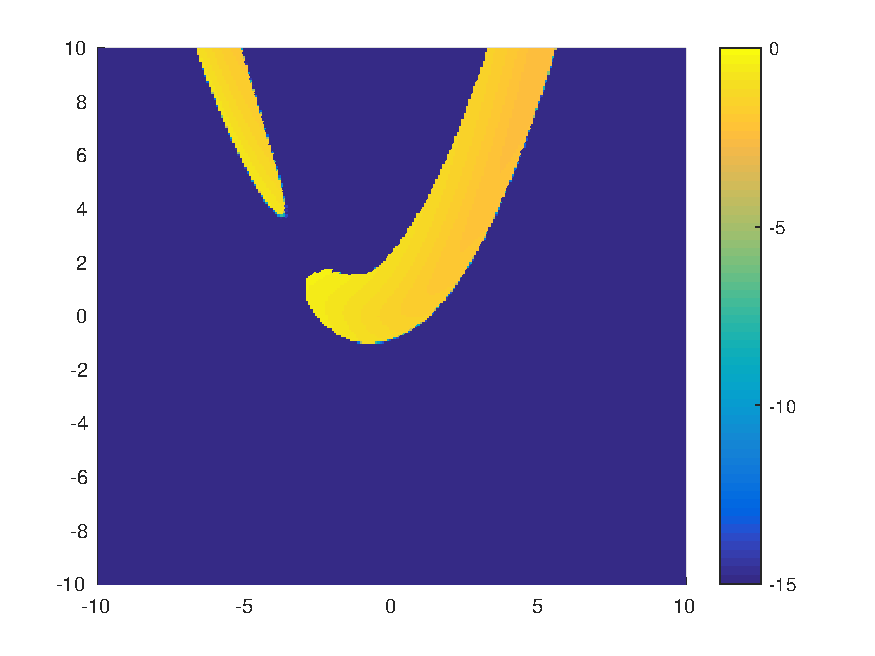
\includegraphics[width=0.45\linewidth]{../src/figure/fig2Matp1}
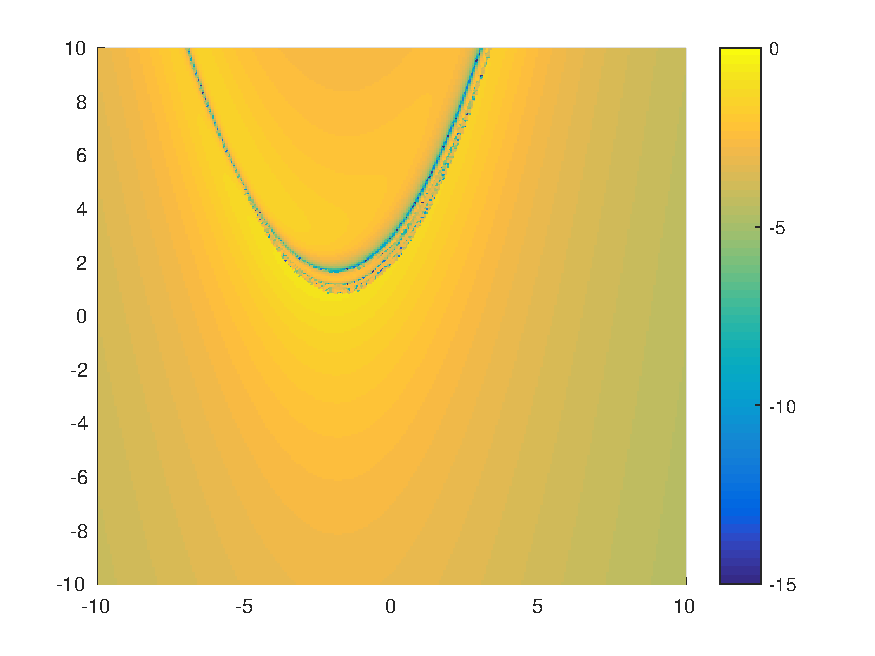
\includegraphics[width=0.45\linewidth]{../src/figure/fig2Matp2}
\caption{Residual magnitude plot for matrix $\mathbf{A}$, as seen in the Embree paper GMRES(1)(left) and GMRES(2)(right) in figure two.}
\label{fig:fig2}
\end{figure}

\begin{figure}
\centering
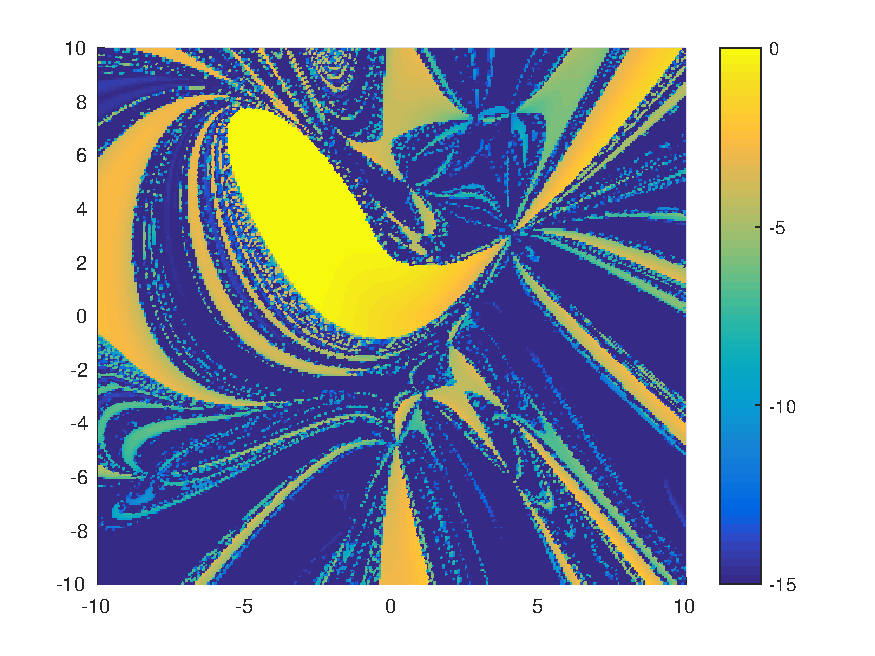
\includegraphics[width=0.45\linewidth]{../src/figure/fig4Matp2}
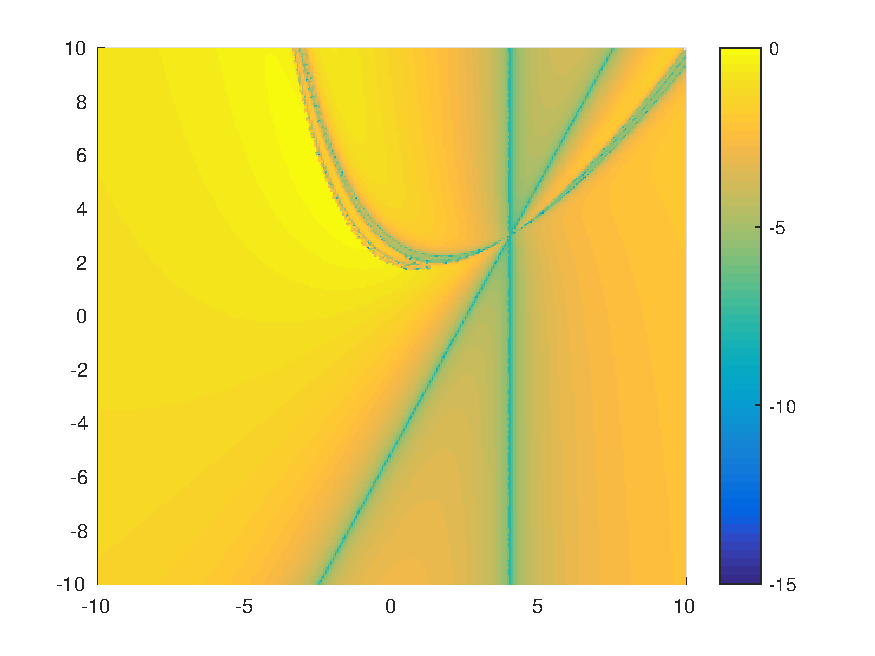
\includegraphics[width=0.45\linewidth]{../src/figure/fig4Matp1}
\caption{Residual magnitude Plot for matrix $\mathbf{B}$, as seen in the Embree paper for GMRES(1)(left) and GMRES(2)(right) in figure 4.}
\label{fig:fig4}
\end{figure}

\subsection{Additional experiments}
If $A - 0.35*\mathbf{I}$ is considered the condition number changes from $\kappa(\mathbf{A}) = 14.2950$ to  $\kappa(\mathbf{A} - 0.35*\mathbf{I}) = 39.1873$. At the same time the convergent area of \texttt{GMRES(1)} shown in figure~\ref{fig:modA}, shrinks considerably in comparison to the plot~\ref{fig:fig2}. Additionally as the conditioning worsened the white foggy areas without convergence grew significantly. 
\begin{figure}
\centering
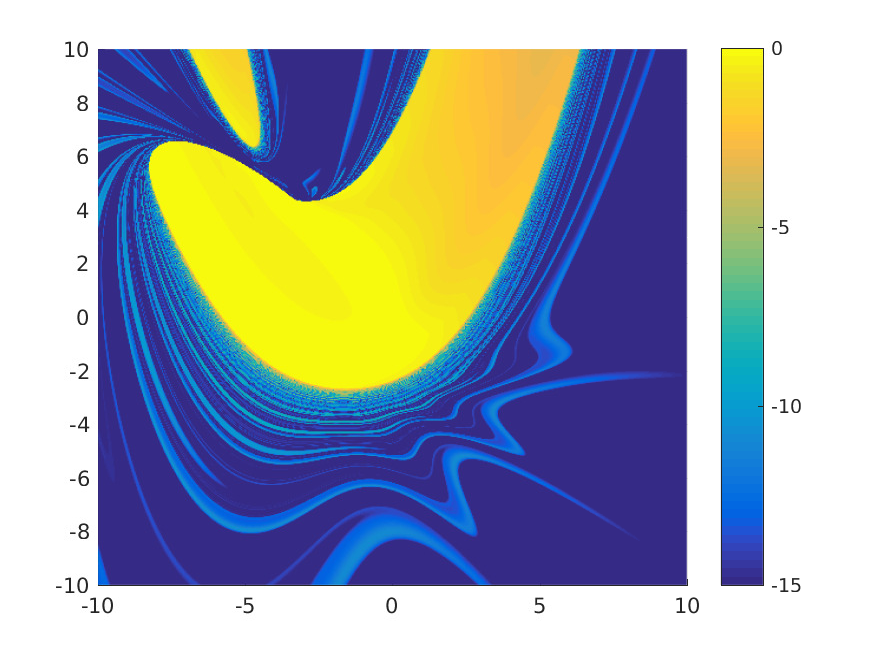
\includegraphics[width=0.45\linewidth]{../src/figure/Am0p35eyeGMRES1}
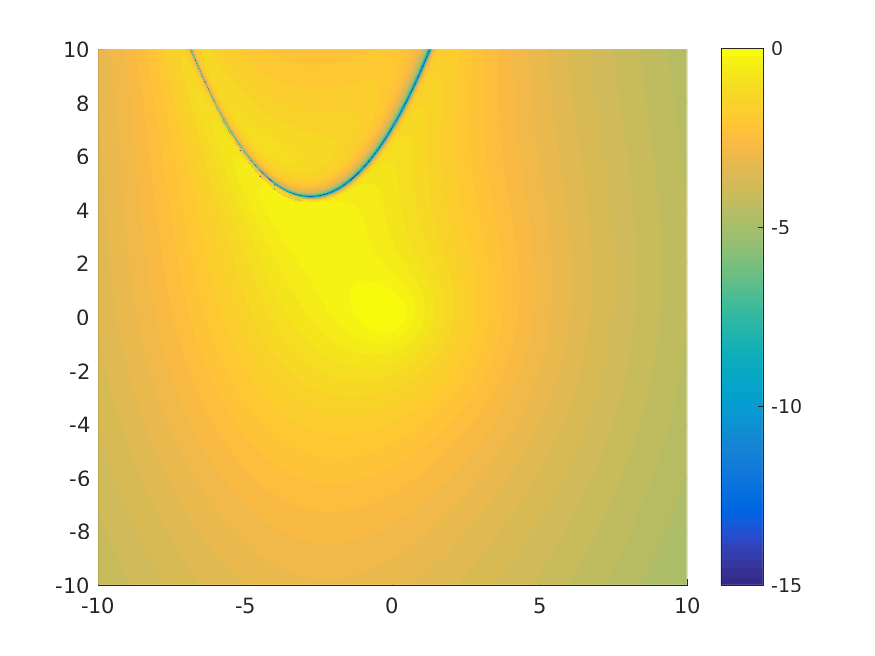
\includegraphics[width=0.45\linewidth]{../src/figure/Am0p35eyeGMRES2}
\caption{\texttt{GMRES(1)} and \texttt{GMRES(2)} convergence on $\mathbf{A} - 0.35 \cdot \mathbf{I}$.  } 
\label{fig:modA}
\end{figure}

In a second series of experiments, designed to further investigate the effect of changed conditioning, $\mathbf{A}$ will be filled with entries drawn from the standart normal distribution ($\mu = 0$, $\sigma^2 = 1$). The values turned out to be:
\begin{equation}
\mathbf{R} = \begin{pmatrix}
-0.3034 &   0.8884 &  -0.8095 \\
 0.2939 &  -1.1471 &  -2.9443 \\
-0.7873 &  -1.0689 &   1.4384 \\
\end{pmatrix} 
\end{equation}
Results for \texttt{GMRES(1)} and \texttt{GMRES(2)}. Are shown in figure \ref{fig:randAGMRES2}. Here it can be observed, that \texttt{GMRES(2)}, converges for all possible right hand sides $\mathbf{b}$, while \texttt{GMRES(1)} does not. This is probably the more common, but mathematically less interesting case. Often convergence improves significantly if the identity matrix is added to A. Unfortunately the condition number got worse by adding one multiple of the identity. It increased from $\kappa(\mathbf{R})=5.1025$ to $\kappa(\mathbf{R} + \mathbf{I})=32.4770$. Adding two times the identity matrix makes matters even worse as $\kappa(\mathbf{R} + 2\mathbf{I})=77.5446$, with results shown in figure~\ref{fig:randAp2eyeGMRES2}. Finally adding three times the identity leads to $\kappa(\mathbf{R} + 3\mathbf{I})=6.4262$ and complete convergence for both algorithms figure~\ref{fig:randAp3eyeGMRES2}. However the conditioning is still worse then it was originally, which indicates that conditioning alone cannot be used to predict \texttt{GMRES(m)} convergence. 

\begin{figure}
\centering
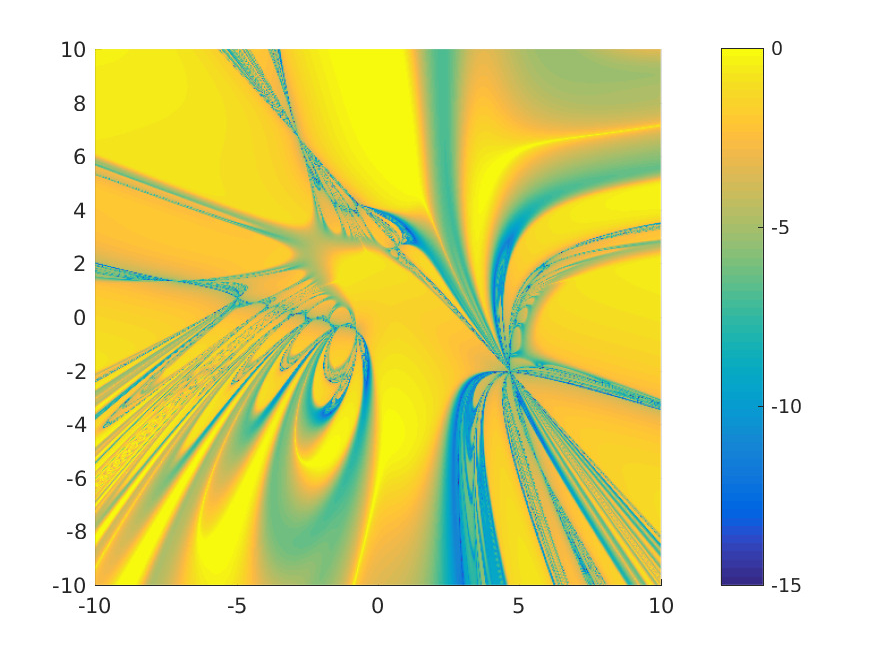
\includegraphics[width=0.45\linewidth]{../src/figure/randAGMRES1}
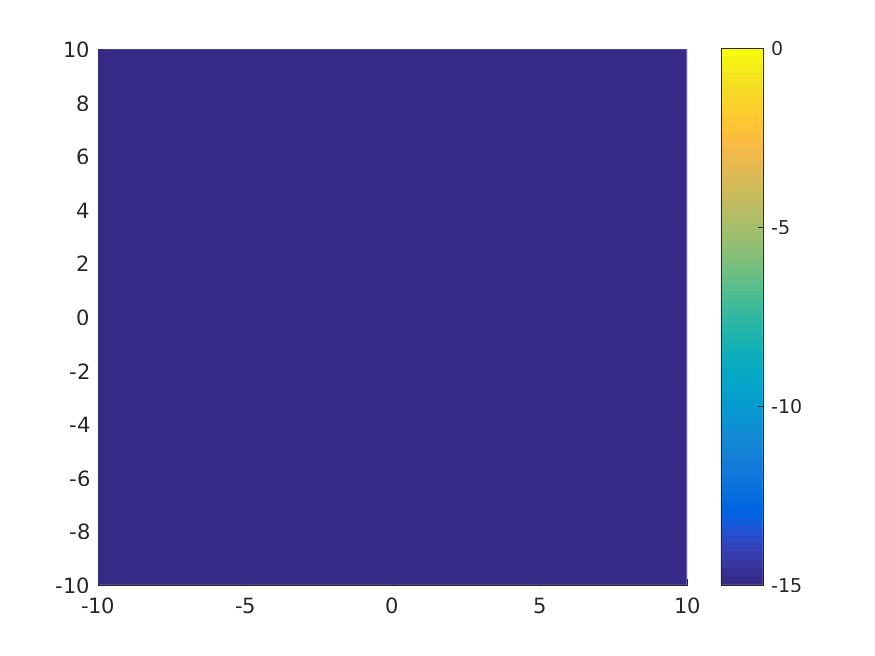
\includegraphics[width=0.45\linewidth]{../src/figure/randAGMRES2}
\caption{Convergence of \texttt{GMRES(1)}(left) and \texttt{GMRES(2)}(right) for the random matrix $\mathbf{R}$.}
\label{fig:randAGMRES2}
\end{figure}
\begin{figure}
\centering
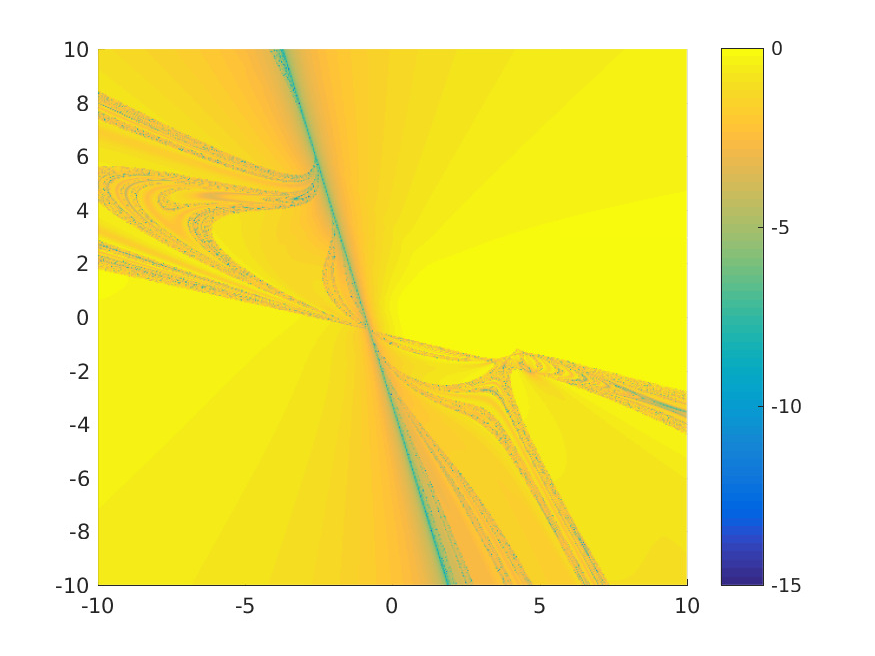
\includegraphics[width=0.45\linewidth]{../src/figure/randAp2eyeGMRES1}
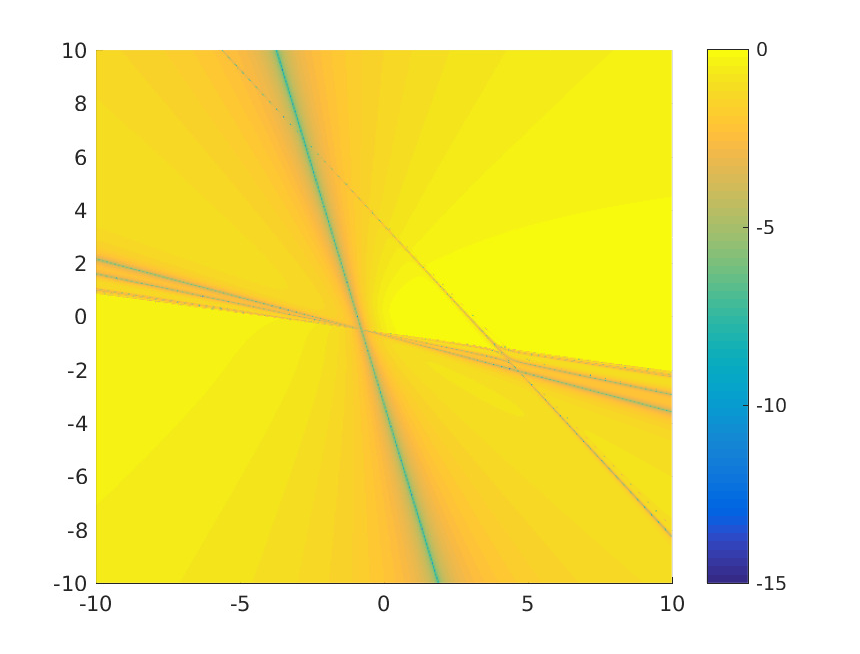
\includegraphics[width=0.45\linewidth]{../src/figure/randAp2eyeGMRES2}
\caption{Convergence results for $\mathbf{R} + 2\mathbf{I}$}
\label{fig:randAp2eyeGMRES2}
\end{figure}
\begin{figure}
\centering
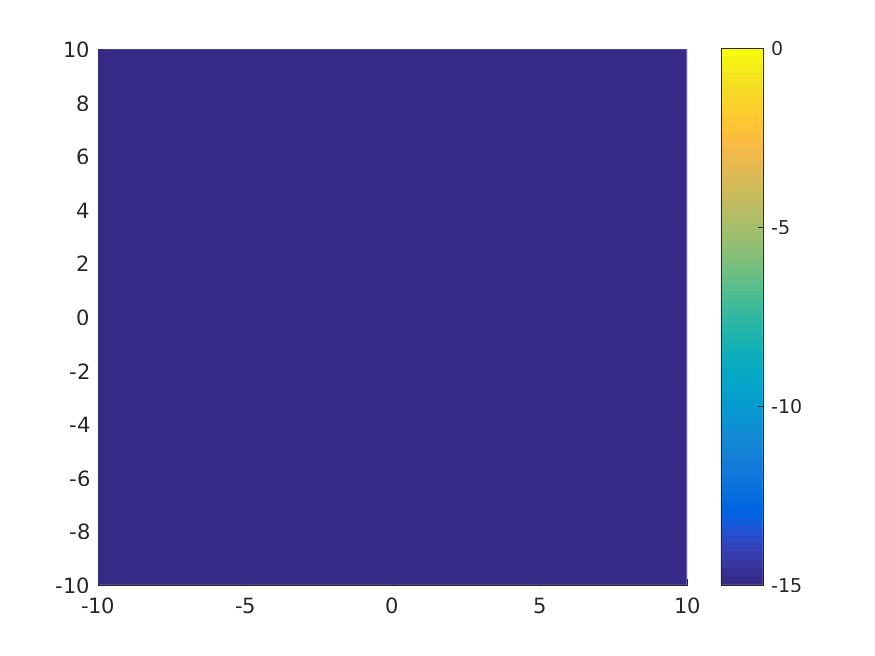
\includegraphics[width=0.45\linewidth]{../src/figure/randAp3eyeGMRES2}
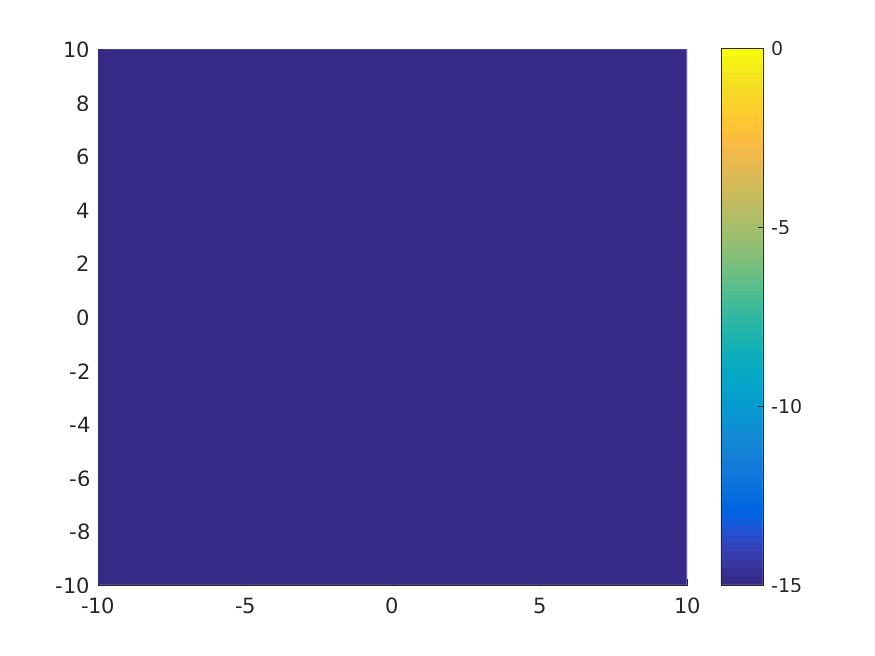
\includegraphics[width=0.45\linewidth]{../src/figure/randAp3eyeGMRES2}
\caption{Convergence results for $\mathbf{R} + 3\mathbf{I}$}
\label{fig:randAp3eyeGMRES2}
\end{figure}

\subsection{Two-Dimensional case}
At the end of the paper Embree proposes to take a closer look at:
\begin{equation}
\mathbf{C} = \begin{pmatrix}
1 & -2 \\
0 & 1 \\
\end{pmatrix}
\;\;\;
\mathbf{r_0} = \begin{pmatrix} \xi \\ \eta \end{pmatrix}
\end{equation}
The residuals show noisy convergence patterns in the bottom and top corners for \texttt{GMRES(1)} in figure~\ref{fig:fig4}. On the right side seemingly random patterns are shown at larger magnification.
Similar ones appeared in figure \ref{fig:fig4} when zooming in. No plot exists for \texttt{GMRES(2)} is it always converged completely within two iterations. In fact for all of the approximately ten two by two matrices that where tried did \texttt{GMRES(2)} converge to the exact result.

\begin{figure}
\centering
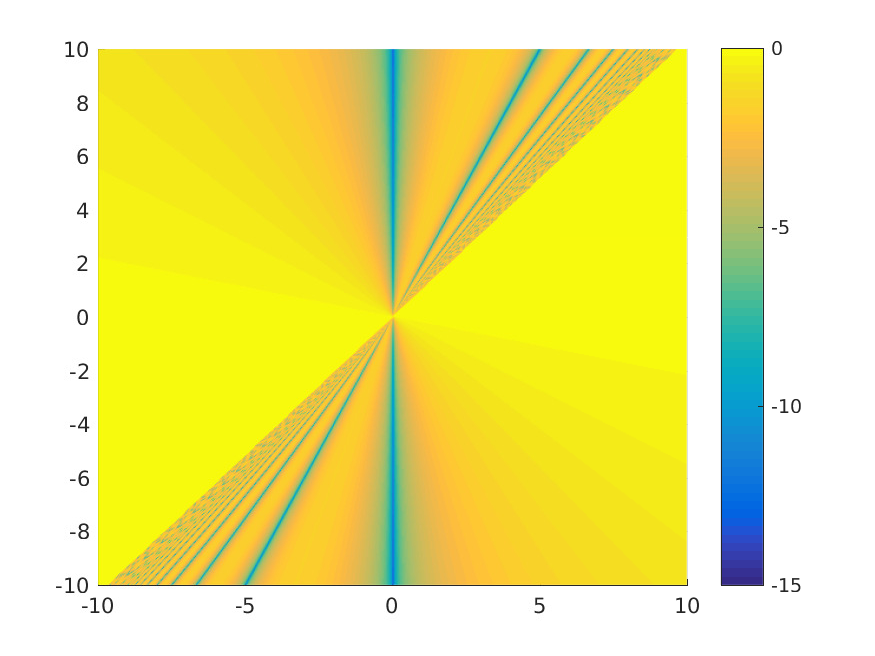
\includegraphics[width=0.45\linewidth]{../src/figure/twoDPaper}
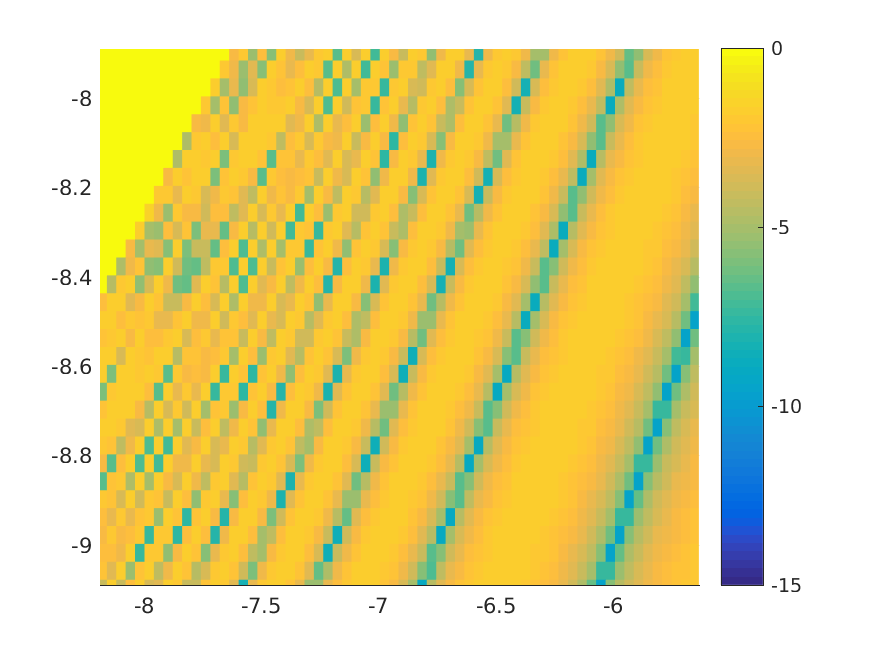
\includegraphics[width=0.45\linewidth]{../src/figure/twoDZoom}
\caption{A plot of the convergence plain for the matrix $\mathbf{C}$ proposed at the end of Embree's paper. With zoom on an interesting region.}
\label{fig:twoDZoom}
\end{figure}

\subsection{An attempt to learn more about the noise.}
In the zoom on figure~\ref{fig:twoDZoom} reveals a noisy area where the outcome of running restart gmres cannot be predicted. This section aims at learning more about the noise. In a first attempt a histogram of the residual magnitude shown in figure~\ref{fig:gmresCHist}, has been made. On the right a zoom on the bottom right part of the histogram is shown, such that parts of the line at zero are neglected. The bar at zero is therefore considerably higher then the one shown. However as most of the surface plot is colored in yellow which corresponds to an error size of $10^0$, this does not come as a surprise that in a histogram of the same image the line at $10^0$. It is rather of more interest do consider the distribution of errors smaller then $10^0 = 1$. And here another peak is observed in bin $[-1.7 -1.6]$, which creates the impression that the noise consists of two superposed noise distribution. As shown in figure~\ref{fig:randnHist} noise with a similar distribution can be produced by superposing shifted absolute valued normal distributions. Finally~\ref{fig:gmresBHist} shows a histogram for the residuals found in the convergence plain of matrix $\mathbf{B}$, interestingly it seems to consists of three superposed distribution. A link between matrix dimensions can not be confirmed by a histogram of $\mathbf{A}$ which only displays two very large bins like $\mathbf{C}$ does.

\begin{figure}
\centering
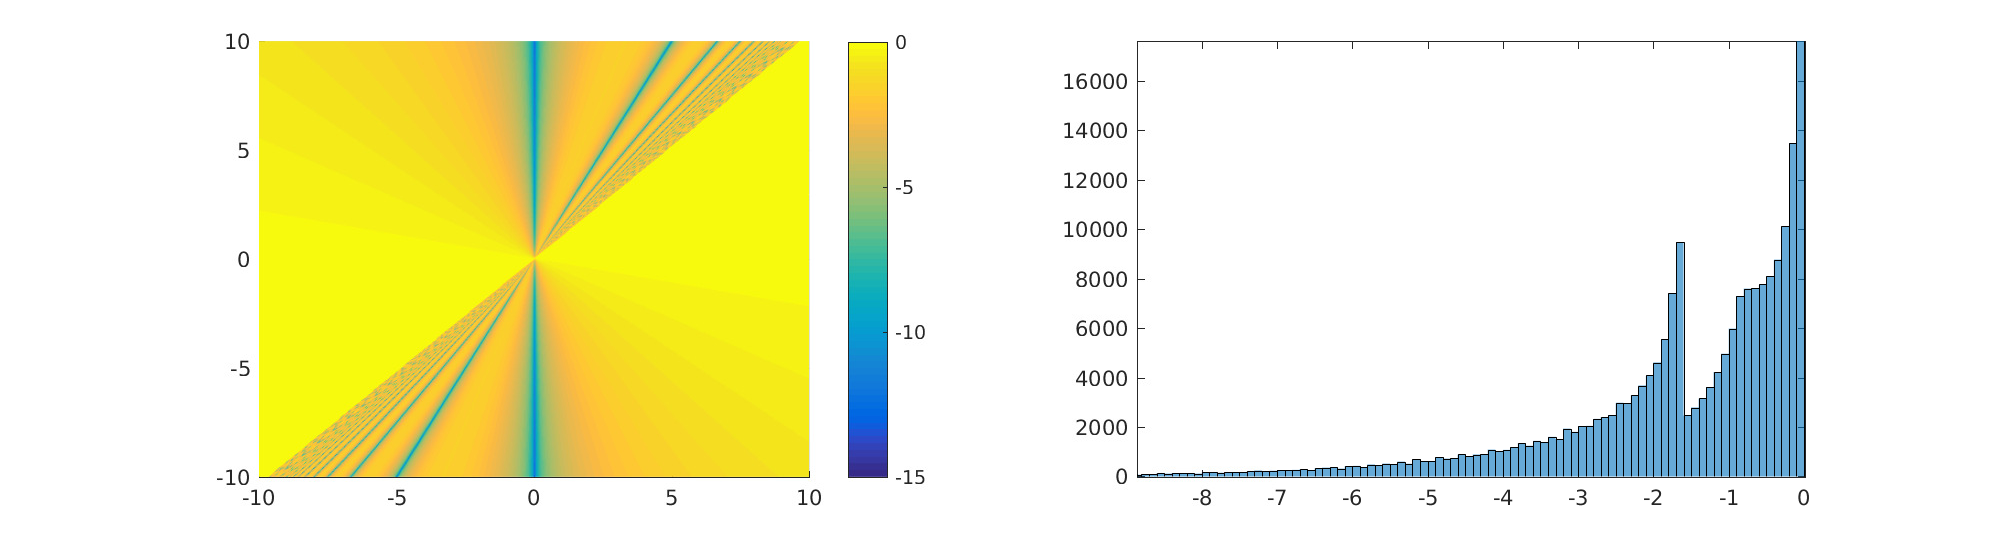
\includegraphics[width=1.05\linewidth]{../src/figure/gmresCHist}
\caption{Convergence plain of matrix $\mathbf{C}$ along with a histogram of the logarithm of the residual norm.}
\label{fig:gmresCHist}
\end{figure}
\begin{figure}
\centering
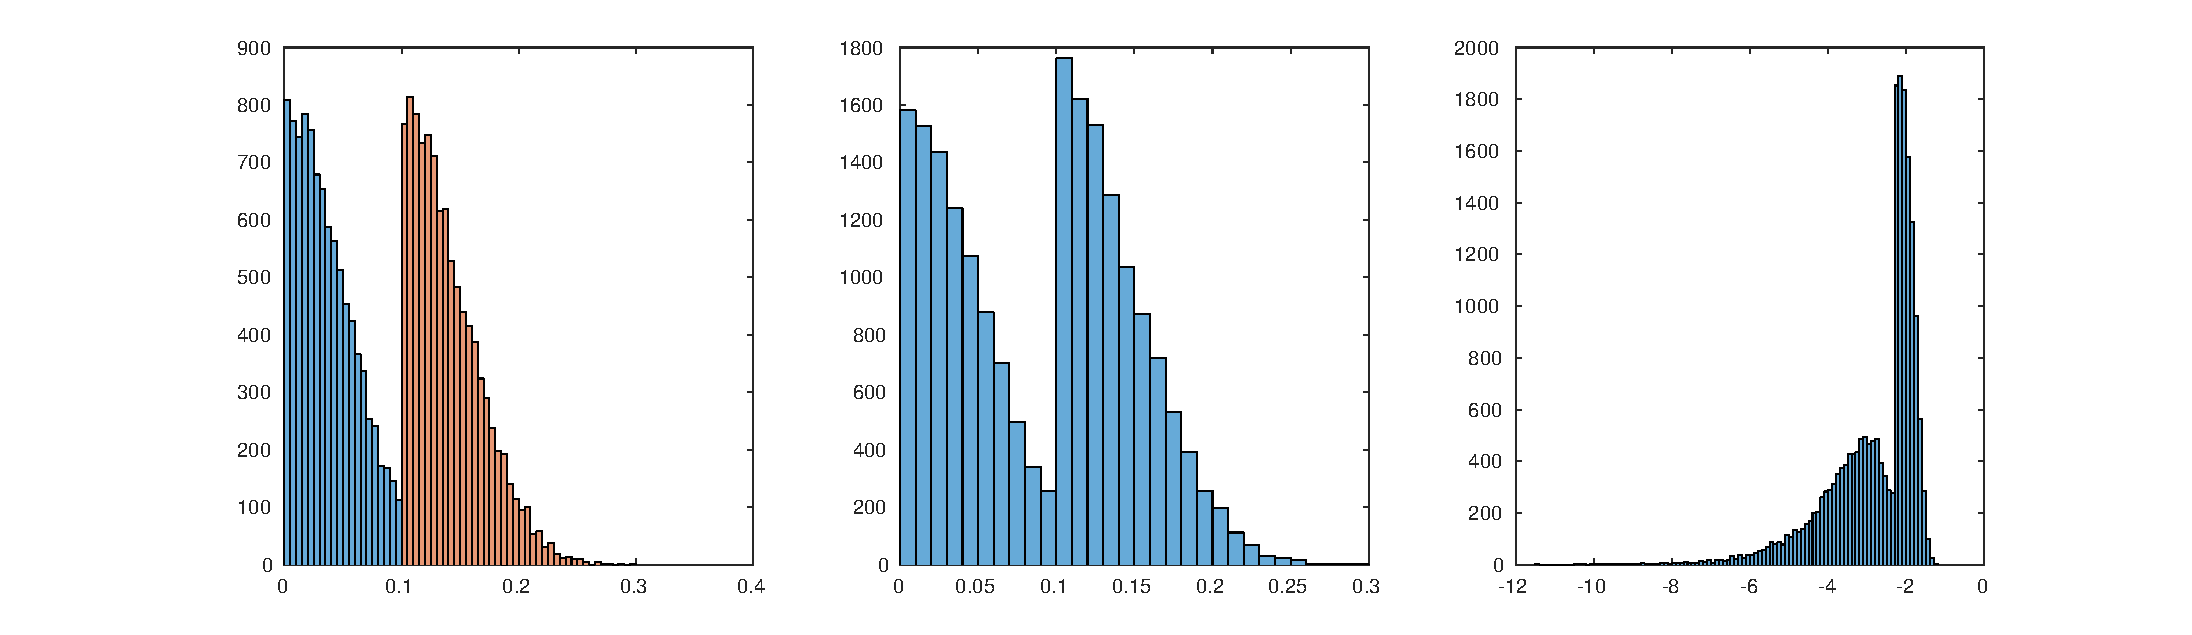
\includegraphics[width=1.05\linewidth]{../src/figure/randnHist}
\caption{Plots of the distributions generated by
\texttt{d1 = 0.00001 + 0.05*abs(randn(10000,1));
d2 = 0.1 + 0.05*abs(randn(10000,1));} . The last plot is on a semilogarithmic scale. }
\label{fig:randnHist}
\end{figure}
\begin{figure}
\centering
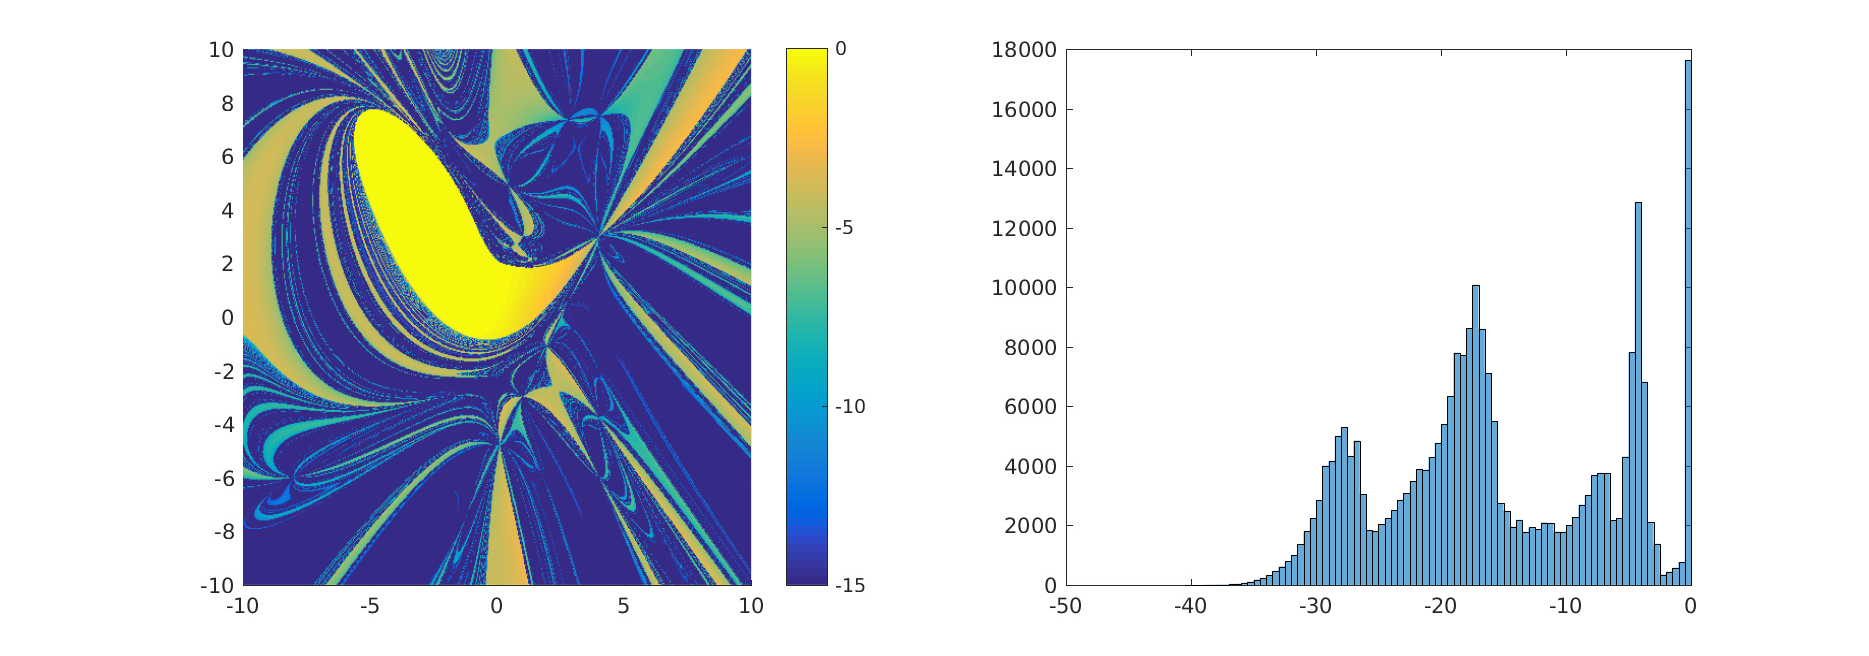
\includegraphics[width=1.05\linewidth]{../src/figure/gmresBHist}
\caption{Convergence plain of matrix $\mathbf{C}$ along with a histogram of the logarithm of the residual norm.}
\label{fig:gmresBHist}
\end{figure}

\subsection{Stagnation condition}
Using the recurrence relation for \texttt{gmres(1)}
\begin{equation}
\mathbf{r}_{k+1}^{(1)} = \mathbf{r}_{k}^{(1)} - \frac{\mathbf{r}_{k}^{(1)T}\mathbf{A}\mathbf{r}_{k}^{(1)}}{\mathbf{r}_{k}^{(1)T}\mathbf{A}^{T}\mathbf{A}\mathbf{r}_{k}^{(1)}} \mathbf{A}\mathbf{r}_{k}^{(1)},
\end{equation}
with $\mathbf{r}_{0} = (\xi \; \eta \; 1)$ it follows that \texttt{gmres(1)} must stagnate if $\mathbf{r}_{k}^{(1)T}\mathbf{A}\mathbf{r}_{k}^{(1)} = 0$. Using the condition above the two elpsoids
\begin{align}
\xi^2 + \xi \eta + \xi + \eta^2 + 3\eta + 1 = 0, \\
\xi^2 + 2\xi \eta -2\xi + 2\eta^2 + 4\eta + 3 = 0
\end{align}
can be found. Which is a set of points on which the algorithms stagnates.
\begin{figure}
\centering
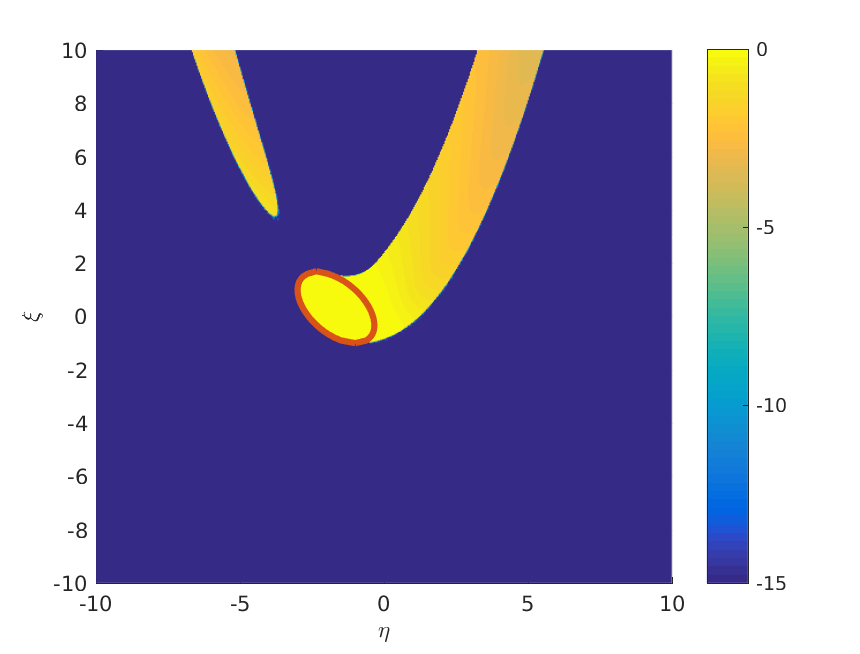
\includegraphics[width=0.45\linewidth]{../src/figure/gmresOneConvA}
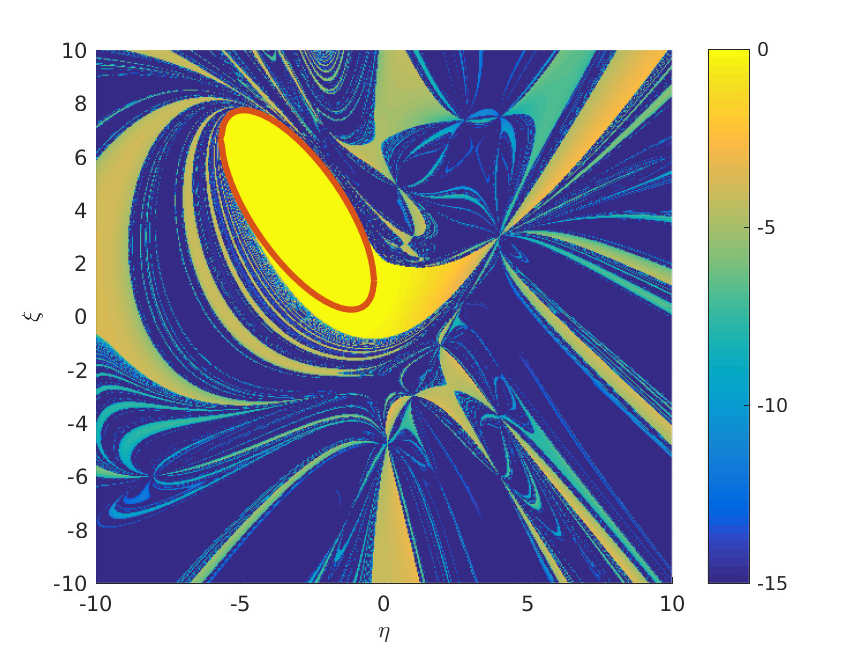
\includegraphics[width=0.45\linewidth]{../src/figure/gmresOneConvB}
\caption{}
\label{fig:gmresOneConv}
\end{figure}



